%!TEX TS-program = xelatex
\documentclass[11pt]{article}

\usepackage[english]{babel}

\usepackage{amsmath,amssymb,amsfonts}
\usepackage[utf8]{inputenc}
\usepackage[T1]{fontenc}
\usepackage{stix}
\usepackage[scaled]{helvet}
\usepackage[scaled]{inconsolata}

\usepackage{lastpage}

\usepackage{setspace}

\usepackage{ccicons}

\usepackage[hang,flushmargin]{footmisc}

\usepackage{geometry}

\setlength{\parindent}{0pt}
\setlength{\parskip}{6pt plus 2pt minus 1pt}

\usepackage{fancyhdr}
\renewcommand{\headrulewidth}{0pt}\providecommand{\tightlist}{%
  \setlength{\itemsep}{0pt}\setlength{\parskip}{0pt}}

\makeatletter
\newcounter{tableno}
\newenvironment{tablenos:no-prefix-table-caption}{
  \caption@ifcompatibility{}{
    \let\oldthetable\thetable
    \let\oldtheHtable\theHtable
    \renewcommand{\thetable}{tableno:\thetableno}
    \renewcommand{\theHtable}{tableno:\thetableno}
    \stepcounter{tableno}
    \captionsetup{labelformat=empty}
  }
}{
  \caption@ifcompatibility{}{
    \captionsetup{labelformat=default}
    \let\thetable\oldthetable
    \let\theHtable\oldtheHtable
    \addtocounter{table}{-1}
  }
}
\makeatother

\usepackage{array}
\newcommand{\PreserveBackslash}[1]{\let\temp=\\#1\let\\=\temp}
\let\PBS=\PreserveBackslash

\usepackage[breaklinks=true]{hyperref}
\hypersetup{colorlinks,%
citecolor=blue,%
filecolor=blue,%
linkcolor=blue,%
urlcolor=blue}
\usepackage{url}

\usepackage{caption}
\setcounter{secnumdepth}{0}
\usepackage{cleveref}

\usepackage{graphicx}
\makeatletter
\def\maxwidth{\ifdim\Gin@nat@width>\linewidth\linewidth
\else\Gin@nat@width\fi}
\makeatother
\let\Oldincludegraphics\includegraphics
\renewcommand{\includegraphics}[1]{\Oldincludegraphics[width=\maxwidth]{#1}}

\usepackage{longtable}
\usepackage{booktabs}

\usepackage{color}
\usepackage{fancyvrb}
\newcommand{\VerbBar}{|}
\newcommand{\VERB}{\Verb[commandchars=\\\{\}]}
\DefineVerbatimEnvironment{Highlighting}{Verbatim}{commandchars=\\\{\}}
% Add ',fontsize=\small' for more characters per line
\usepackage{framed}
\definecolor{shadecolor}{RGB}{248,248,248}
\newenvironment{Shaded}{\begin{snugshade}}{\end{snugshade}}
\newcommand{\KeywordTok}[1]{\textcolor[rgb]{0.13,0.29,0.53}{\textbf{#1}}}
\newcommand{\DataTypeTok}[1]{\textcolor[rgb]{0.13,0.29,0.53}{#1}}
\newcommand{\DecValTok}[1]{\textcolor[rgb]{0.00,0.00,0.81}{#1}}
\newcommand{\BaseNTok}[1]{\textcolor[rgb]{0.00,0.00,0.81}{#1}}
\newcommand{\FloatTok}[1]{\textcolor[rgb]{0.00,0.00,0.81}{#1}}
\newcommand{\ConstantTok}[1]{\textcolor[rgb]{0.00,0.00,0.00}{#1}}
\newcommand{\CharTok}[1]{\textcolor[rgb]{0.31,0.60,0.02}{#1}}
\newcommand{\SpecialCharTok}[1]{\textcolor[rgb]{0.00,0.00,0.00}{#1}}
\newcommand{\StringTok}[1]{\textcolor[rgb]{0.31,0.60,0.02}{#1}}
\newcommand{\VerbatimStringTok}[1]{\textcolor[rgb]{0.31,0.60,0.02}{#1}}
\newcommand{\SpecialStringTok}[1]{\textcolor[rgb]{0.31,0.60,0.02}{#1}}
\newcommand{\ImportTok}[1]{#1}
\newcommand{\CommentTok}[1]{\textcolor[rgb]{0.56,0.35,0.01}{\textit{#1}}}
\newcommand{\DocumentationTok}[1]{\textcolor[rgb]{0.56,0.35,0.01}{\textbf{\textit{#1}}}}
\newcommand{\AnnotationTok}[1]{\textcolor[rgb]{0.56,0.35,0.01}{\textbf{\textit{#1}}}}
\newcommand{\CommentVarTok}[1]{\textcolor[rgb]{0.56,0.35,0.01}{\textbf{\textit{#1}}}}
\newcommand{\OtherTok}[1]{\textcolor[rgb]{0.56,0.35,0.01}{#1}}
\newcommand{\FunctionTok}[1]{\textcolor[rgb]{0.00,0.00,0.00}{#1}}
\newcommand{\VariableTok}[1]{\textcolor[rgb]{0.00,0.00,0.00}{#1}}
\newcommand{\ControlFlowTok}[1]{\textcolor[rgb]{0.13,0.29,0.53}{\textbf{#1}}}
\newcommand{\OperatorTok}[1]{\textcolor[rgb]{0.81,0.36,0.00}{\textbf{#1}}}
\newcommand{\BuiltInTok}[1]{#1}
\newcommand{\ExtensionTok}[1]{#1}
\newcommand{\PreprocessorTok}[1]{\textcolor[rgb]{0.56,0.35,0.01}{\textit{#1}}}
\newcommand{\AttributeTok}[1]{\textcolor[rgb]{0.77,0.63,0.00}{#1}}
\newcommand{\RegionMarkerTok}[1]{#1}
\newcommand{\InformationTok}[1]{\textcolor[rgb]{0.56,0.35,0.01}{\textbf{\textit{#1}}}}
\newcommand{\WarningTok}[1]{\textcolor[rgb]{0.56,0.35,0.01}{\textbf{\textit{#1}}}}
\newcommand{\AlertTok}[1]{\textcolor[rgb]{0.94,0.16,0.16}{#1}}
\newcommand{\ErrorTok}[1]{\textcolor[rgb]{0.64,0.00,0.00}{\textbf{#1}}}
\newcommand{\NormalTok}[1]{#1}

\newlength{\cslhangindent}
\setlength{\cslhangindent}{1.5em}
\newlength{\csllabelwidth}
\setlength{\csllabelwidth}{3em}
\newenvironment{CSLReferences}[3] % #1 hanging-ident, #2 entry spacing
 {% don't indent paragraphs
  \setlength{\parindent}{0pt}
  % turn on hanging indent if param 1 is 1
  \ifodd #1 \everypar{\setlength{\hangindent}{\cslhangindent}}\ignorespaces\fi
  % set entry spacing
  \ifnum #2 > 0
  \setlength{\parskip}{#2\baselineskip}
  \fi
 }%
 {}
\usepackage{calc} % for \widthof, \maxof
\newcommand{\CSLBlock}[1]{#1\hfill\break}
\newcommand{\CSLLeftMargin}[1]{\parbox[t]{\maxof{\widthof{#1}}{\csllabelwidth}}{#1}}
\newcommand{\CSLRightInline}[1]{\parbox[t]{\linewidth}{#1}}
\newcommand{\CSLIndent}[1]{\hspace{\cslhangindent}#1}\geometry{verbose,letterpaper,tmargin=2.5cm,bmargin=2.5cm,lmargin=2.5cm,rmargin=4.5cm}

\usepackage{lineno}
\usepackage[nolists,noheads]{endfloat}

\pagestyle{plain}

\doublespacing

\fancypagestyle{normal}
{
  \fancyhf{}
  \fancyfoot[R]{\footnotesize\sffamily\thepage\ of \pageref*{LastPage}}
}
\begin{document}
\thispagestyle{empty}
{\Large\bfseries\sffamily A Roadmap Toward Predicting Species
Interaction Networks (Across Space and Time)}
\vskip 5em

%
\href{https://orcid.org/0000-0001-6067-1349}{Tanya\,Strydom}%
%
\,\textsuperscript{1,2,‡}\quad %
\href{https://orcid.org/0000-0002-6506-6487}{Michael D.\,Catchen}%
%
\,\textsuperscript{3,2,‡}\quad %
\href{https://orcid.org/0000-0001-9051-0597}{Francis\,Banville}%
%
\,\textsuperscript{1,4,2}\quad %
\href{https://orcid.org/0000-0002-2151-6693}{Dominique\,Caron}%
%
\,\textsuperscript{3,2}\quad %
\href{https://orcid.org/0000-0002-2212-3584}{Gabriel\,Dansereau}%
%
\,\textsuperscript{1,2}\quad %
\href{https://orcid.org/0000-0002-6248-3007}{Philippe\,Desjardins-Proulx}%
%
\,\textsuperscript{1,2}\quad %
\href{https://orcid.org/0000-0001-9019-0108}{Norma R.\,Forero-Muñoz}%
%
\,\textsuperscript{1,2}\quad %
\href{https://orcid.org/0000-0003-2791-8383}{Gracielle\,Higino}%
%
\,\textsuperscript{5}\quad %
\href{https://orcid.org/0000-0002-4104-9463}{Benjamin\,Mercier}%
%
\,\textsuperscript{4,2}\quad %
\href{https://orcid.org/0000-0001-6075-8081}{Andrew\,Gonzalez}%
%
\,\textsuperscript{3,2}\quad %
\href{https://orcid.org/0000-0002-4498-7076}{Dominique\,Gravel}%
%
\,\textsuperscript{4,2}\quad %
\href{https://orcid.org/0000-0002-6004-4027}{Laura\,Pollock}%
%
\,\textsuperscript{3,2}\quad %
\href{https://orcid.org/0000-0002-0735-5184}{Timothée\,Poisot}%
%
\,\textsuperscript{1,2}

\textsuperscript{1}\,Université de
Montréal\quad \textsuperscript{2}\,Québec Centre for Biodiversity
Sciences\quad \textsuperscript{3}\,McGill
University\quad \textsuperscript{4}\,Université de
Sherbrooke\quad \textsuperscript{5}\,Universidade Federal de Goiás

\textsuperscript{‡}\,These authors contributed equally to the work\\

\textbf{Correspondance to:}\\
Timothée Poisot --- \texttt{timothee.poisot@umontreal.ca}\\

\vfill
This work is released by its authors under a CC-BY 4.0 license\hfill\ccby\\
Last revision: \emph{\today}

\clearpage
\thispagestyle{empty}

\vfill
\textbf{\sffamily Abstract: }Networks of species interactions underpin
numerous ecosystem processes, but comprehensively sampling these
interactions is difficult. Interactions intrinsically vary across space
and time, and given the number of species that compose ecological
communities, it can be tough to distinguish between a true negative
(where two species never interact) from a false negative (where two
species have not been observed interacting even though they actually
do). Assessing the likelihood of interactions between species is an
imperative for several fields of ecology. This means that to predict
interactions between species---and to describe the structure, variation,
and change of the ecological networks they form---we need to rely on
modeling tools. Here we provide a proof-of-concept, where we show how a
simple neural-network model makes accurate predictions about species
interactions given limited data. We then assess the challenges and
opportunities associated with improving interaction predictions, and
provide a conceptual roadmap forward toward predictive models of
ecological networks that is explicitly spatial and temporal. We conclude
with a brief primer on the relevant methods and tools needed to start
building these models, which we hope will guide this research program
forward.
\vfill

\clearpage
\linenumbers
\pagestyle{normal}

\hypertarget{introduction}{%
\section{Introduction}\label{introduction}}

Ecosystems are, in large part, constructed by the interactions within
them --- organisms interact with one-another and with their environment,
either directly or indirectly. Interactions between individuals,
populations, and species create networks of interactions that drive
ecological and evolutionary dynamics and maintain the coexistence,
diversity, and functioning of ecosystems (Delmas et al. 2018; Landi et
al. 2018; Albrecht et al. 2018). Species interaction networks underpin
our understanding of numerous ecological processes (Pascual and Dunne
2006; Heleno et al. 2014). Yet, even basic knowledge of species
interactions (like being able to list them, or guess which ones may
exist) remains one of the most severe biodiversity shortfalls (Hortal et
al. 2015), in large part due to the tedious, time-consuming, and
expensive process of collecting species interaction data.
Comprehensively sampling every possible interaction is not feasible
given the sheer number of species on Earth, and the data we can collect
about interactions tend to be biased and noisy (de Aguiar et al. 2019).
This is then compounded as species interactions are typically measured
as a binary variable (present or absent) even though it is evident
interactions are not all-or-nothing. Empirically we know species
interactions occur probabilistically due to variation in species
abundances in space and time (Poisot, Stouffer, and Gravel 2015).
Different types of interactions vary in their intrinsic predictability
(e.g.~some fungal species engage in opportunistic saprotrophy (Smith et
al. 2017), obligate parasites are more deterministic in their
interactions than facultative parasites (Poisot et al. 2013; Luong and
Mathot 2019)). In addition to this variance in predictability, networks
from different systems are structured by different mechanisms.

Still, like all of Earth's systems, species interaction networks have
entered their ``long now'' (Carpenter 2002), where anthropogenic change
will have long-term, low-predictability consequences (Burkle, Marlin,
and Knight 2013) for our planet's ecology. Therefore, our field needs a
roadmap towards models that enable prediction (for the present) and
forecasting (for the future) of species interactions and the networks
they form, and which accounts for their spatial and temporal variation
(McCann 2007; Seibold et al. 2018). As an example, in disease ecology,
predicting potential hosts of novel disease (recently notably the search
for wildlife hosts of betacoronaviruses; Becker et al. 2020; Wardeh,
Baylis, and Blagrove 2021) has received much attention. Network
approaches have been used for the prediction of risk and dynamics of
dengue (Zhao et al. 2020), Chagas disease (Rengifo-Correa et al. 2017),
Rickettsiosis (Morand et al. 2020), Leishmaniasis (Stephens 2009), and a
myriad infectious diseases in livestock and wildlife (Craft 2015).
Additionally, prediction of interaction networks is a growing imperative
for next-generation biodiversity monitoring, requiring a conceptual
framework and a flexible set of tools to predict interactions that is
explicitly spatial and temporal in perspective (Edwards et al. 2021;
Magioli and Ferraz 2021; Zhang and He 2021). Developing better models
for prediction of these interactions will rely on integration of data
from many sources, and the sources for this data may differ depending on
the type of interaction we wish to predict (Gibb et al. 2021).

Interactions between species can be conceptualised in a multitude of
ways (mutualistic vs.~antagonistic, strong vs.~weak, symmetric
vs.~asymmetric, direct vs.~indirect) (Jordano 2016a; Morales-Castilla et
al. 2015). What is common among definitions of species interactions is
that \emph{at least} one of the species is affected by the presence of
another (Morales-Castilla et al. 2015). Networks can be used to
represent a variety of interaction types, including: \emph{unipartite
networks}: where each species can be linked to other species (often food
webs), \emph{bipartite networks}: where there are two pools of species
and all interactions occur between species in each pool (typically used
for pairwise interactions; e.g.~hosts and parasites), and
\emph{k-partite networks,}: which expand to more than two discrete sets
of interacting species (e.g., some parasitoid webs, seed dispersal
networks, and pollination networks (Pocock, Evans, and Memmott 2012)).

Methods for predicting interactions between species exist, but at the
moment are difficult to generalise as they are typically based around a
single mechanism at a single scale: position in the trophic niche
(Gravel et al. 2013; Petchey et al. 2008), phylogenetic distance
(Pomeranz et al. 2018; Elmasri et al. 2020), functional trait matching
(Bartomeus et al. 2016), interaction frequency (Weinstein and Graham
2017; Vázquez, Morris, and Jordano 2005), or other network properties
(Terry and Lewis 2020; Stock et al. 2017). Species interaction networks,
as we observe them on Earth today, are the product of ecological and
evolutionary mechanisms interacting across spatial, temporal and
organisational scales. The interwoven nature of these processes imposes
structure on biodiversity data which is invisible when examined only
through the lens of a single scale, however machine learning (ML)
methods have enormous potential to find this structure in data
(Desjardins-Proulx, Poisot, and Gravel 2019), and have the potential to
be used together with mechanistic models in order to make prediction of
ecological dynamics more robust (Rackauckas et al. 2020).

Here we use a case study to show how machine-learning models
(specifically a deep neural network) can enable prediction of species
interactions: we construct a metaweb of host-parasite interactions
across space, using predictors extracted from empirical data and
accounting for the structure of co-occurrence between species. We use
this case study to illustrate a roadmap for improving predictions using
open data and ML methods; specifically, we focus on how emerging tools
from ML can be used to deliver more accurate and more efficient
predictions of ecological systems, and how the potential of these
approaches will be magnified with increased data access. We then provide
a non-exhaustive primer on the literature on interaction prediction, and
identify the tools and methods most suited for the future of interaction
network prediction models, covering the spatial, temporal, and climatic
dimensions of network prediction (Burkle and Alarcon 2011). Both the
case study and primer are largely geared towards binary (interactions
are either present or absent) networks; there are limitations in data
and tools that make it a more reasonable starting approach. First, most
ecological networks do not have estimates of interaction strength, and
particularly not estimates that are independent from relative
abundances. Second, the methodological toolkit to analyse the structure
of networks is far more developed for binary interactions (Delmas et al.
2018), meaning that the predictions of binary interactions can be more
readily interpreted.

We argue that adopting a more predictive approach to complex ecological
systems (like networks) will establish a positive feedback loop with our
understanding of these systems (Houlahan et al. 2017): the tasks of
understanding and predicting are neither separate nor opposed (Maris et
al. 2017); instead, ML tools have the ability to capture a lot of our
understanding into working assumptions, and comparing predictions to
empirical data gives us better insights about how much we ignore about
the systems we model (see for example Borowiec et al. 2021, who provide
an overview of deep learning techniques and concepts in ecology and
evolution). Although data on species interaction networks are currently
limited in the size and spatial coverage, machine learning approaches
have a demonstrated track record of revealing the ``unreasonable
effectiveness'' of data (Halevy, Norvig, and Pereira 2009); we argue
that with a clear roadmap guiding the use of these methods, the task of
predicting species interaction networks will become more attainable.

\hypertarget{a-case-study-deep-learning-of-spatially-sparse-host-parasite-interactions}{%
\section{A case study: deep learning of spatially sparse host-parasite
interactions}\label{a-case-study-deep-learning-of-spatially-sparse-host-parasite-interactions}}

The premise of this manuscript is that we can predict interactions
between species. In this section we provide a proof-of-concept, where we
use data from Hadfield et al. (2014) describing 51 host-parasite
networks sampled across space. In this data, as in most spatially
distributed ecological networks, not all species co-occur across sites.
As a direct consequence there are pairs of species that may or may not
be able to interact for which we have no data; furthermore there are
pairs of species that may interact, but have only been documented in a
single location where the interaction was not detected. In short, there
are ecological reasons to believe that a number of negative associations
in the metaweb (\emph{sensu} J. Dunne 2006) are false negatives.

Without any species-level information, we resort to using both
co-occurrence and known interactions to predict novel interactions. To
do this we (i) extract features (equivalent to explanatory variables in
a statistical model) for each species based on co-occurrence, (ii) use
these features to train an artificial neural network to predict
interactions, and (iii) apply this classifier (an algorithm that assigns
a categorical output based on input features) to the original features
to predict potential interactions across the entire species pool.
Machine learning relies on a lexicon that shares some terms with
statistics, albeit with different meaning; we expand on the precise
meanings in the ``How to validate a predictive model'' section below.
The outputs of the analysis are presented in fig.~\ref{fig:example}, and
the code to reproduce it is available at \texttt{https://osf.io/6jp4b/};
the entire example was carried out in \emph{Julia 1.6.2} (Bezanson et
al. 2017), using the \emph{Flux} machine learning framework (Innes
2018).

We first aggregate all species into a co-occurrence matrix \(A\) which
represents whether a given pair of species \((i,j)\) was observed
coexisting across any location. We then transform this co-occurrence
matrix \(A\) via probabilistic PCA (Tipping and Bishop 1999) and use the
first 15 values from this PCA space as the features vector for each
species \(i\). For each pair of (host, parasite) species \((i,j)\), we
then feed the features vectors \((v_i, v_j)\) into a neural network. The
neural network uses four feed-forward layers (each layer is independent
from the one before and after); the first layer uses the \(\text{RELU}\)
activation function (which ignores input below a threshold), the rest
use a \(\sigma\) function (which transforms linear activation energies
into logistic responses). All layers have appropriate dropout rates (in
order to avoid over-fitting, only a fraction of the network is updated
on each iteration: \(1-0.8\) for the first layer, \(1-0.6\) for the
subsequent ones). This produces an output layer with a single node,
which is the probability-score for interaction between species \(i\) and
\(j\).

We then train (equivalent to \emph{fit}) this neural network by dividing
the original dataset into testing and training sets (split 80-20 for
training and testing respectively). During the training of this neural
network (using the ADAM optimiser), the \(5\times 10^4\) batches of 64
items used for training were constrained to have at least 25\% of
positive interactions, as Poisot, Ouellet, et al. (2021) show slightly
inflating the dataset with positive interactions enables us to
counterbalance sampling biases. Furthermore, setting a minimum threshold
of response balance is an established approach for datasets with strong
biases (Lemaître, Nogueira, and Aridas 2017). Validating this model on
the test data shows our model provides highly effective prediction of
interactions between pairs of species not present in the training data
(fig.~\ref{fig:example}). The behaviour of the model was, in addition,
checked by measuring the training and testing loss (difference between
the actual value and the prediction, here using mean-squared error) and
stopping well before they diverged (to avoid overfitting).

\begin{figure}
\hypertarget{fig:example}{%
\centering
\includegraphics{figures/figure1.png}
\caption{Proof-of-Concept: An empirical metaweb (from Hadfield et al.
2014), i.e.~a list of known possible interactions within a species pool,
is converted into latent features using probabilistic PCA, then used to
train a deep neural network to predict species interactions. Panels A
and B represent, respectively, the ROC curve and the precision-recall
curve, with the best classifier (according to Youden's J) represented by
a black dot. The expected performance of a neutral ``random-guessing''
classifier is shown with a dashed line. Panel C shows the imputed using
t-distributed stochastic neighbour embedding (tSNE), and the colours of
nodes are the cluster to which they are assigned based on a \(k\)-means
clustering of the tSNE output. Empirical interactions are shown in
purple, and imputed interactions in grey.}\label{fig:example}
}
\end{figure}

This case study shows that a simple neural network can be very effective
in predicting species interactions even without additional species-level
data. Applying this model to the entire dataset (including species pairs
never observed to co-occur) identified 1546 new possible interactions --
746 (48\%) of which were between pairs of species for which no
co-occurrence was observed in the original dataset. This model reaches
similar levels of predictive efficacy as previous studies that use far
more species-level data and mechanistic assumptions (Gravel et al.
2013), which serves to highlight the potential for including external
sources of data for \emph{improving} our prediction of interaction
networks even further. For example, Krasnov et al. (2016) collected
traits data for this system that could be added to the model, in
addition or in substitution to latent variables derived from observed
interactions.

\hypertarget{predicting-species-interaction-networks-across-space-challenges-and-opportunities}{%
\section{Predicting species interaction networks across space:
challenges and
opportunities}\label{predicting-species-interaction-networks-across-space-challenges-and-opportunities}}

Here we present a conceptual roadmap (fig.~\ref{fig:conceptual}) which
shows a conceptual path from data to prediction of species interaction
networks, incorporating several modelling frameworks. We envisage this
roadmap to be one conceptual path toward incorporating space in to our
prediction of interaction networks, and developing spatially explicit
models of networks and their properties. In the following sections we
discuss the challenges and opportunities for this path forward, and
highlight two specific areas where it can have a strong impact: the
temporal forecasting of species interaction networks structure, and the
use of predicted networks for applied ecology and conservation biology.

\begin{figure}
\hypertarget{fig:conceptual}{%
\centering
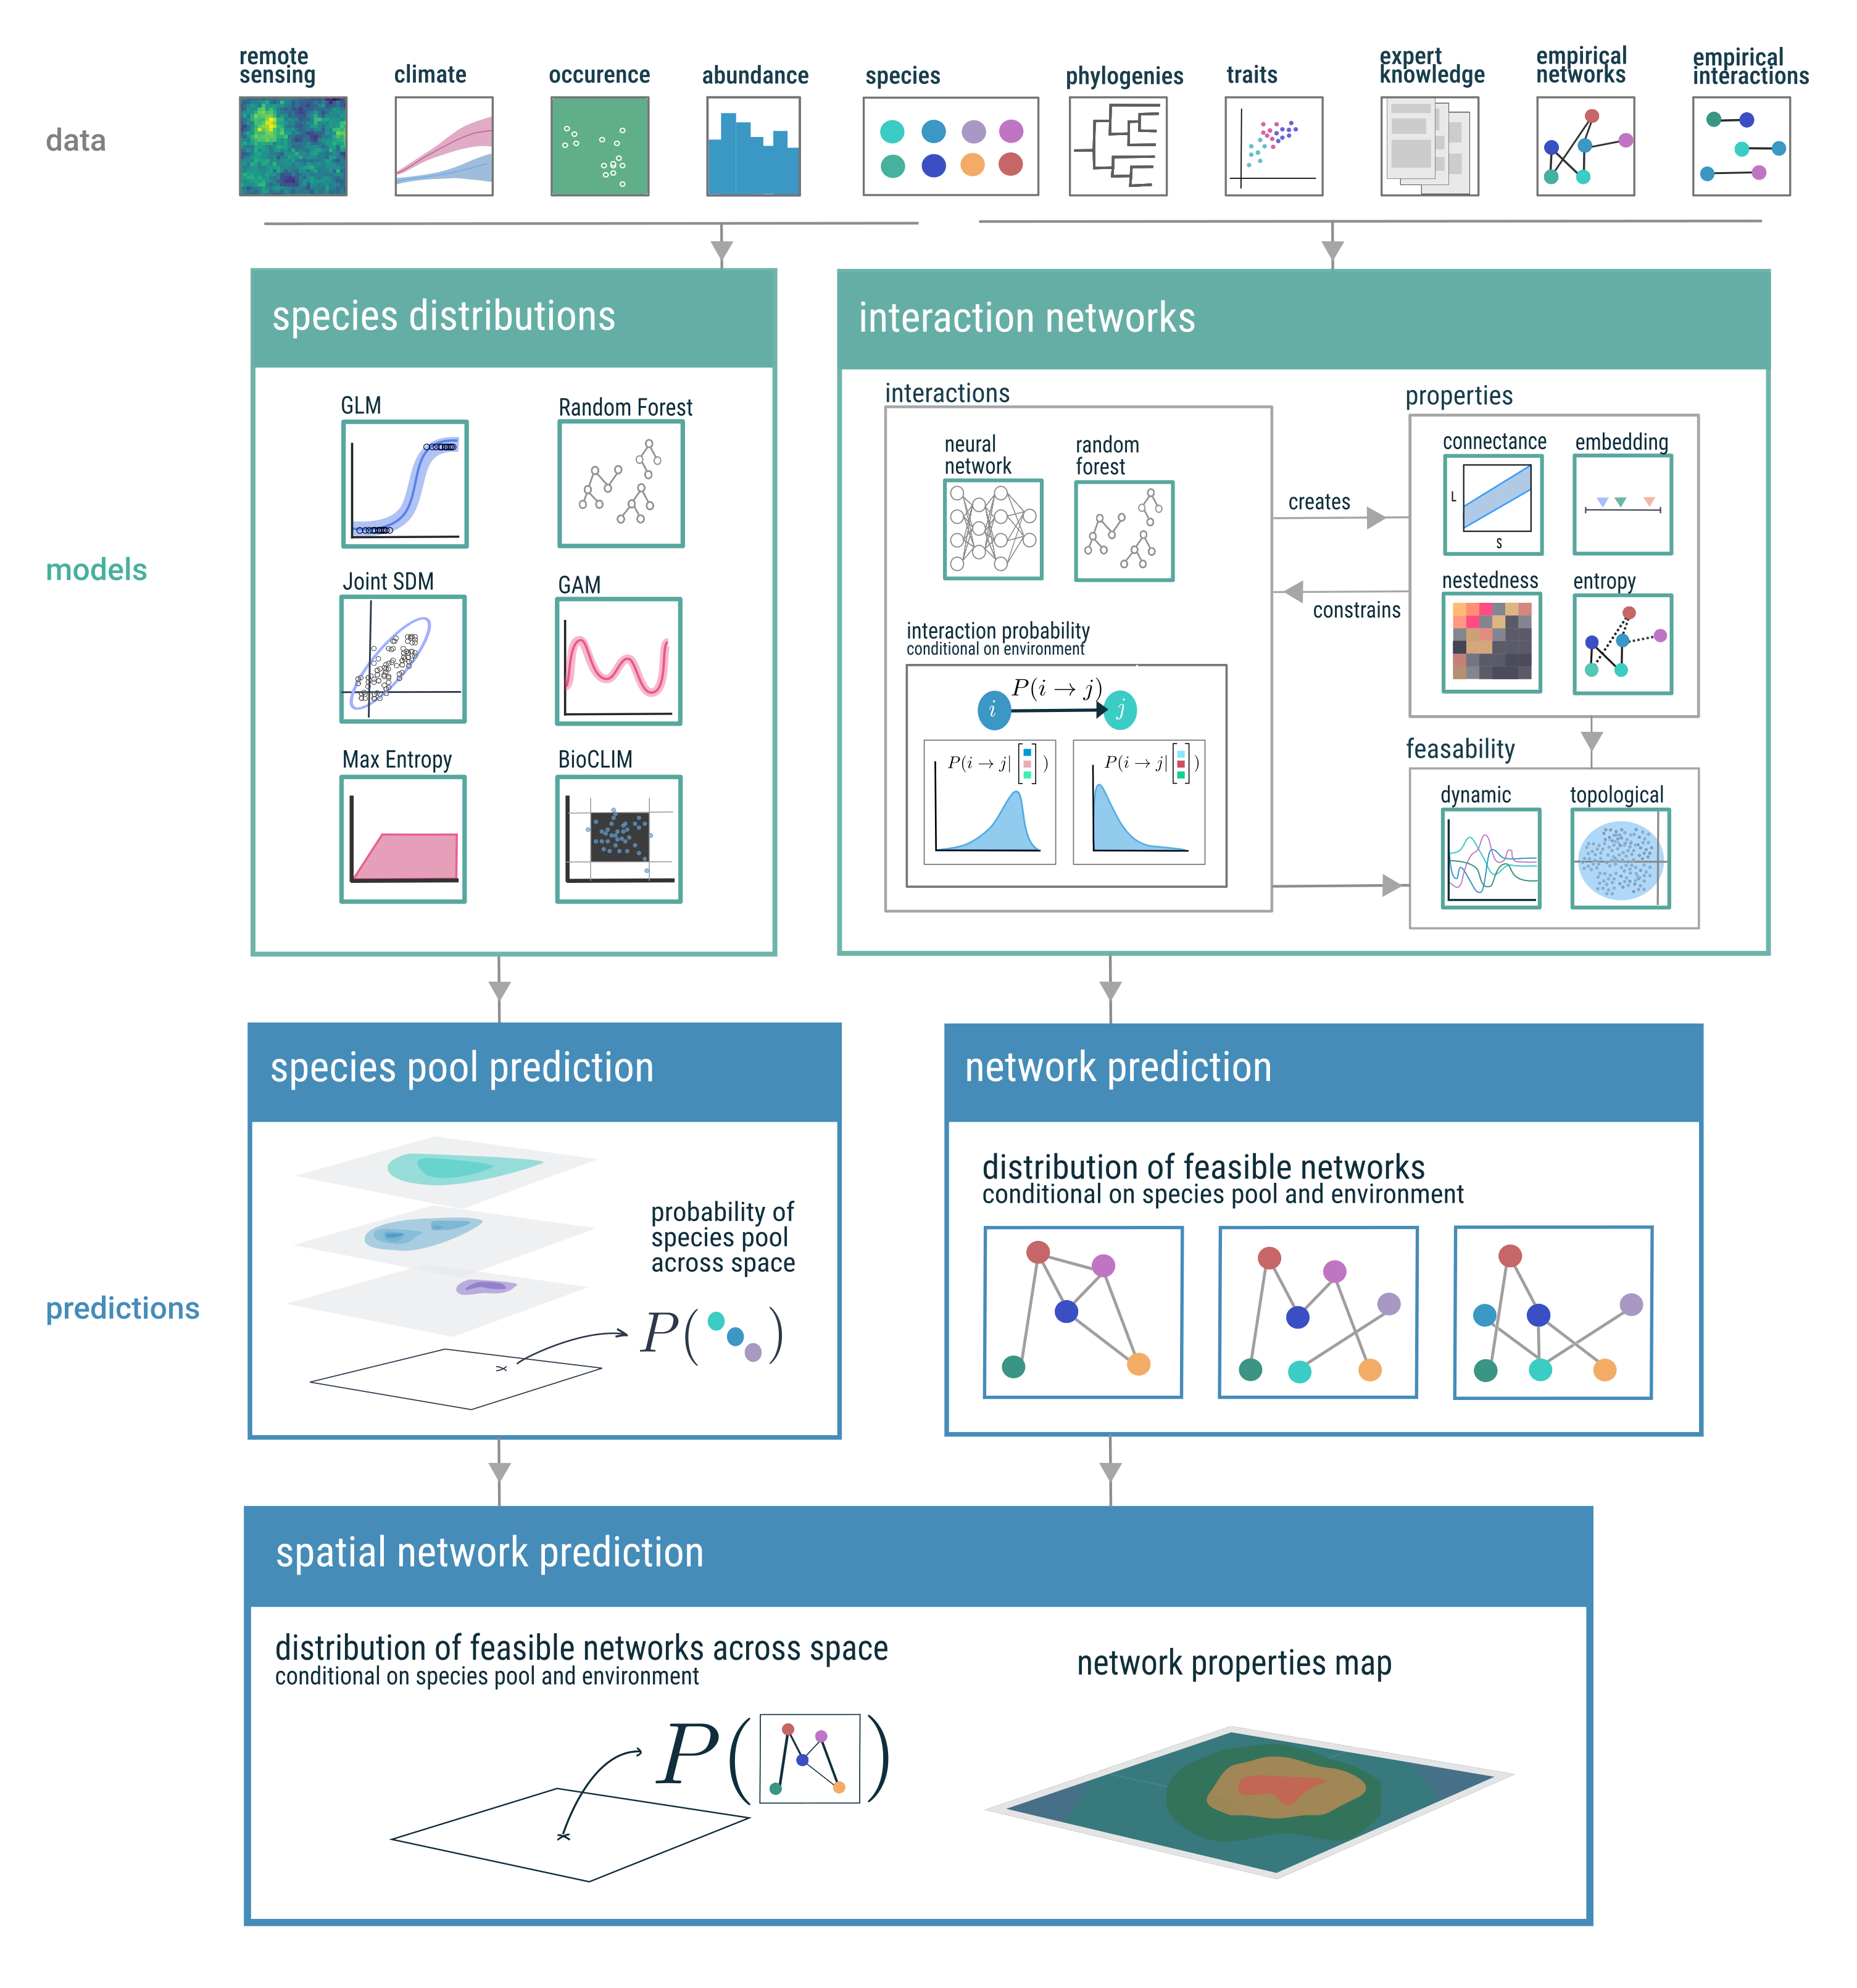
\includegraphics{figures/concept_v6.png}
\caption{A conceptual roadmap highlighting key areas for the prediction
of ecological networks. Starting with the input of data from multiple
sources, followed by a modelling framework for ecological networks and
the landscape, which are then ultimately combined to allow for the
prediction of spatially explicit networks.}\label{fig:conceptual}
}
\end{figure}

\hypertarget{challenges-constraints-on-predictions}{%
\subsection{Challenges: constraints on
predictions}\label{challenges-constraints-on-predictions}}

\hypertarget{ecological-network-data-are-scarce-and-hard-to-obtain}{%
\subsubsection{Ecological network data are scarce and hard to
obtain}\label{ecological-network-data-are-scarce-and-hard-to-obtain}}

At the moment, prediction of species interactions is made difficult by
the limited availability of data. Although we have seen a growth in
species occurrence data, this growth is much slower for ecological
interactions because species interactions are challenging to sample
comprehensively (Bennett, Evans, and Powell 2019; Jordano 2016b) and
sampling methodology has strong effects on the resulting data (de Aguiar
et al. 2019). In turn, the difficulty of sampling interactions can lead
to biases in our understanding of network structure (de Aguiar et al.
2019). This knowledge gap has motivated a variety of approaches to deal
with interactions in ecological research based on assumptions that do
not always hold, such as the assumption that co-occurrence is equivalent
to meaningful interaction strength (Blanchet, Cazelles, and Gravel
2020). Spatial biases in data coverage are prevalent at the global scale
(with South America, Africa and Asia being under-represented) and
different interaction types show biases towards different biomes
(Poisot, Bergeron, et al. 2021). These ``spatial gaps'' serve as a
limitation to our ability to confidently make predictions when
accounting for real-world environmental conditions, especially in
environments for which there are no analogous data.

Further, empirical estimation of interaction \emph{strength} is highly
prone to bias as existing data are usually summarised at the taxonomic
scale of the species or higher, thereby losing information that
differentiates the strength in per-individual interactions from the
strength of a whole species interaction (Wells and O'Hara 2013).
Empirical estimations of interaction strength are still crucial (Novak
and Wootton 2008), but are a hard task to quantify in natural
communities (Wootton 1997; Sala and Graham 2002; Wootton and Emmerson
2005), especially as the number of species composing communities
increases, compounded by the possibility of higher-order interactions or
non-linear responses in interactions (Wootton and Emmerson 2005).
Further, interaction strength is often variable and context dependent
and can be influenced by density-dependence and spatio-temporal
variation in community composition (Wootton and Emmerson 2005).

\hypertarget{powerful-predictive-tools-work-better-on-large-data-volumes}{%
\subsubsection{Powerful predictive tools work better on large data
volumes}\label{powerful-predictive-tools-work-better-on-large-data-volumes}}

This scarcity of data limits the range of computational tools that can
be used by network ecologists. Most deep learning methods, for instance,
are very data expensive. The paucity of data is compounded by a
collection of biases in existing datasets. Species interaction data are
typically dominated by food webs, pollination, and host-parasite
networks (Ings et al. 2009; Poisot et al. 2020). This could prove to be
a limiting factor when trying to understand or predict networks of
underrepresented interaction types or when trying to integrate networks
of different types (Fontaine et al. 2011), especially given their
inherent structural variation (Michalska-Smith and Allesina 2019). This
stresses the need for an integrated, flexible, and data-efficient set of
computational tools which will allow us to predict ecological networks
accurately from existing and imperfect datasets, but also enable us to
perform model validation and comparison with more flexibility than
existing tools. We argue that fig.~\ref{fig:example} is an example of
the promise of these tools \emph{even} when facing datasets of small
size. The ability to extract and engineer features also serves to
bolster our predictive power. Although it may be tempting to rely on
approaches like bootstrapping to estimate the consistency of the
predictions, we are confronted with the issues of low data volume and
data bias---that we are more likely to observe interactions between some
pairs of species (i.e.~those that co-occur often, e.g. Cazelles et al.
(2015), and those with higher relative abundance, e.g. Vazquez et al.
(2009)). This introduces risk in training models on pseudo-replicated
data. In short, the current lack of massive datasets must not be an
obstacle to prediction; it is an ideal testing ground to understand how
little data is sufficient to obtain actionable predictions, and how much
we can rely on data inflation procedures to reach this minimal amount.

\hypertarget{scaling-up-predictions-requires-scaled-up-data}{%
\subsubsection{Scaling-up predictions requires scaled-up
data}\label{scaling-up-predictions-requires-scaled-up-data}}

We are also currently limited by the level of biological organisation at
which we can describe ecological networks. For instance, our
understanding of individual-based networks (e.g., M. S. Araújo et al.
2008; Tinker et al. 2012) is still in its infancy (Guimarães 2020) and
acts as a resolution-limit. Similarly, the resolution of environmental
(or landscape) data also limits our ability to predict networks at small
scales, although current trends in remote sensing would suggest that
this will become less of a hindrance with time (Makiola et al. 2020).
Ecosystems are a quintessential complex-adaptive-system (Levin 1998)
with a myriad of processes at different spatial, temporal, and
organisational scales that influence and respond to one another.
Understanding how the product of these different processes drive the
properties of ecosystems across different scales remains a central
challenge of ecological research, and we should strive to work on
methods that will integrate different empirical ``snapshots'' of this
larger system.

\hypertarget{opportunities-an-emerging-ecosystem-of-open-tools-and-data}{%
\subsection{Opportunities: an emerging ecosystem of open tools and
data}\label{opportunities-an-emerging-ecosystem-of-open-tools-and-data}}

\hypertarget{data-are-becoming-more-interoperable}{%
\subsubsection{Data are becoming more
interoperable}\label{data-are-becoming-more-interoperable}}

The acquisition of biodiversity and environmental data has tremendously
increased over the past decades thanks to the rise of citizen science
(J. L. Dickinson, Zuckerberg, and Bonter 2010) and of novel technology
(Stephenson 2020), including wireless sensors (Porter et al. 2005),
next-generation DNA sequencing (Creer et al. 2016), and remote sensing
(Skidmore and Pettorelli 2015; Lausch et al. 2016). Open access
databases, such as \href{https://www.gbif.org/}{GBIF} (for biodiversity
data), \href{https://www.ncbi.nlm.nih.gov/}{NCBI} (for taxonomic and
genomics data),
\href{https://www.treebase.org/treebase-web/home.html}{TreeBASE} (for
phylogenetics data), \href{https://icestes.github.io/}{CESTE} (Jeliazkov
et al. 2020) (for metacommunity ecology and species traits data), and
\href{https://www.worldclim.org/data/bioclim.html}{WorldClim} (for
bioclimatic data) contain millions of data points that can be integrated
to monitor and model biodiversity at the global scale. For species
interactions data, at the moment \href{https://mangal.io/\#/}{Mangal} is
the most comprehensive open database of published ecological networks
(Poisot et al. 2016), and
\href{https://www.globalbioticinteractions.org/about}{GloBI} is an
extensive database of realised and potential species interactions
(Poelen, Simons, and Mungall 2014). Developing standard practices in
data integration and quality control (Kissling et al. 2018) and in
next-generation biomonitoring (NGB; Makiola et al. 2020) would improve
our ability to make reliable predictions of ecosystem properties on
increasing spatial and temporal scales. The advancement of prediction
techniques coupled with a movement towards standardising data collection
protocols (e.g. Pérez-Harguindeguy et al. (2013) for plant functional
traits) and metadata (e.g.
\href{https://www.tdwg.org}{DarwinCore})---which facilitates
interoperability and integration of datasets---as well as a growing
interest at the government level (Scholes et al. 2012) paints a positive
picture for data access and usability in the coming years.

\hypertarget{machine-learning-tools-are-becoming-more-accessible}{%
\subsubsection{Machine learning tools are becoming more
accessible}\label{machine-learning-tools-are-becoming-more-accessible}}

This effort is also supported by a thriving ecosystem of data sources
and novel tools. ML methods can often be more flexible and perform
better than classical statistical methods, and can achieve a very high
level of accuracy in many predictive and classification tasks in a
relatively short amount of time (e.g., Cutler et al. 2007; Krizhevsky,
Sutskever, and Hinton 2017). Increasing computing power combined with
recent advances in machine learning techniques and applications shows
promise in ecology and environmental science (see Christin, Hervet, and
Lecomte (2019) for an overview). Moreover, ongoing developments in deep
learning are aimed at improvement in low-data regimes and with
unbalanced datasets (Antoniou, Storkey, and Edwards 2018; Chawla 2010).
Considering the current biases in network ecology (Poisot, Bergeron, et
al. 2021) and the scarcity of data of species interactions, the
prediction of ecological networks will undoubtedly benefit from these
improvements. Machine learning methods are emerging as the new standard
in computational ecology in general (Olden, Lawler, and Poff 2008;
Christin, Hervet, and Lecomte 2019), and in network ecology in
particular (Bohan et al. 2017), as long as sufficient, relevant data are
available. Many studies have used machine learning models specifically
with ecological interactions. Relevant examples include species traits
used to predict interactions and infer trait-matching rules
(Desjardins-Proulx et al. 2017; Pichler et al. 2020), automated
discovery of food webs (Bohan et al. 2011), reconstruction of ecological
networks using next-generation sequencing data (Bohan et al. 2017), and
network inference from presence-absence data (Sander, Wootton, and
Allesina 2017). As many ecological and evolutionary processes underlie
species interactions and the structure of their ecological networks
(e.g., Vazquez et al. 2009; Segar et al. 2020), it can be difficult to
choose relevant variables and model species interactions networks
explicitly. A promising application of machine learning in natural
sciences is Scientific-Machine Learning (SciML), a framework that
combines machine learning with mechanistic models (Chuang and Keiser
2018; Rackauckas et al. 2020).

\hypertarget{a-primer-on-predicting-ecological-networks}{%
\section{A primer on predicting ecological
networks}\label{a-primer-on-predicting-ecological-networks}}

Within the constraints outlined in the previous section, we now provide
a primer on the background concepts necessary to build predictive models
of species interaction networks, with a focus on using machine learning
approaches in the modelling process. As fig.~\ref{fig:conceptual}
illustrates, this involves a variety of numerical and computational
approaches; therefore, rather than an exhaustive summary, we aim to
convey a high-level understanding that translates the core concepts into
their application to ecological networks.

\hypertarget{models}{%
\subsection{Models}\label{models}}

\hypertarget{what-is-a-predictive-model}{%
\subsubsection{What is a predictive
model?}\label{what-is-a-predictive-model}}

Models are used for many purposes, and the term ``model'' itself
embodies a wide variety of meanings in scientific discourse. All models
can be thought of as a function, \(f\), that takes a set of inputs \(x\)
(also called features, descriptors, or independent variables) and
parameters \(\theta\), and maps them to predicted output states \(y\)
(also called label, response, or dependent variable) based on the input
to the model: \(y=f(x,\theta)\).

A given model \(f\) can be used for either descriptive or predictive
purposes. Many forms of scientific inquiry are based around using models
\emph{descriptively}, a practice also called inference, the inverse
problem, fitting a model, or training a model (Stouffer 2019). In this
context, the goal of using a model is to estimate the parameters,
\(\theta\), that best explain a set of empirical observations,
\(\{\hat{x}, \hat{y}\}\). In some cases, these parameter values are
themselves of interest (e.g., the strength of selection, intrinsic
growth rate, dispersal distance), but in others cases, the goal is to
compare a set of competing models \(f_1, f_2, \dots\) to determine which
provides the most parsimonious explanation for a dataset. The
quantitative representation of ``effects'' in these models---the
influence of each input on the output---is often assumed to be linear,
and within the frequentist world-view, the goal is often to determine if
the coefficient corresponding with an input is non-zero to determine its
``significance'' (often different from its ecological relevance;
Martínez-Abraín 2008) in influencing the outcome.

Models designed for inference have utility---descriptive models of
networks can reveal underlying mechanisms that structure ecological
communities, given a proper null model (Connor, Barberán, and Clauset
2017). However, in order for ecology to develop as a predictive science
(Evans, Norris, and Benton 2012), interest has grown in developing
models that are used not just for description of data, but also for
prediction. Predictive models are based in \emph{the forward problem},
where the aim is to predict new values of the output \(y\) given an
input \(x\) and our estimate value of \(\theta\) (Stouffer 2019).
Because the forward problem relies on an estimate of \(\theta\), then,
the problem of inference is nested within the forward problem
(fig.~\ref{fig:models}): working towards a predictive view of ecological
networks will give us the needed tools to further our understanding of
them.

\begin{figure}
\hypertarget{fig:models}{%
\centering
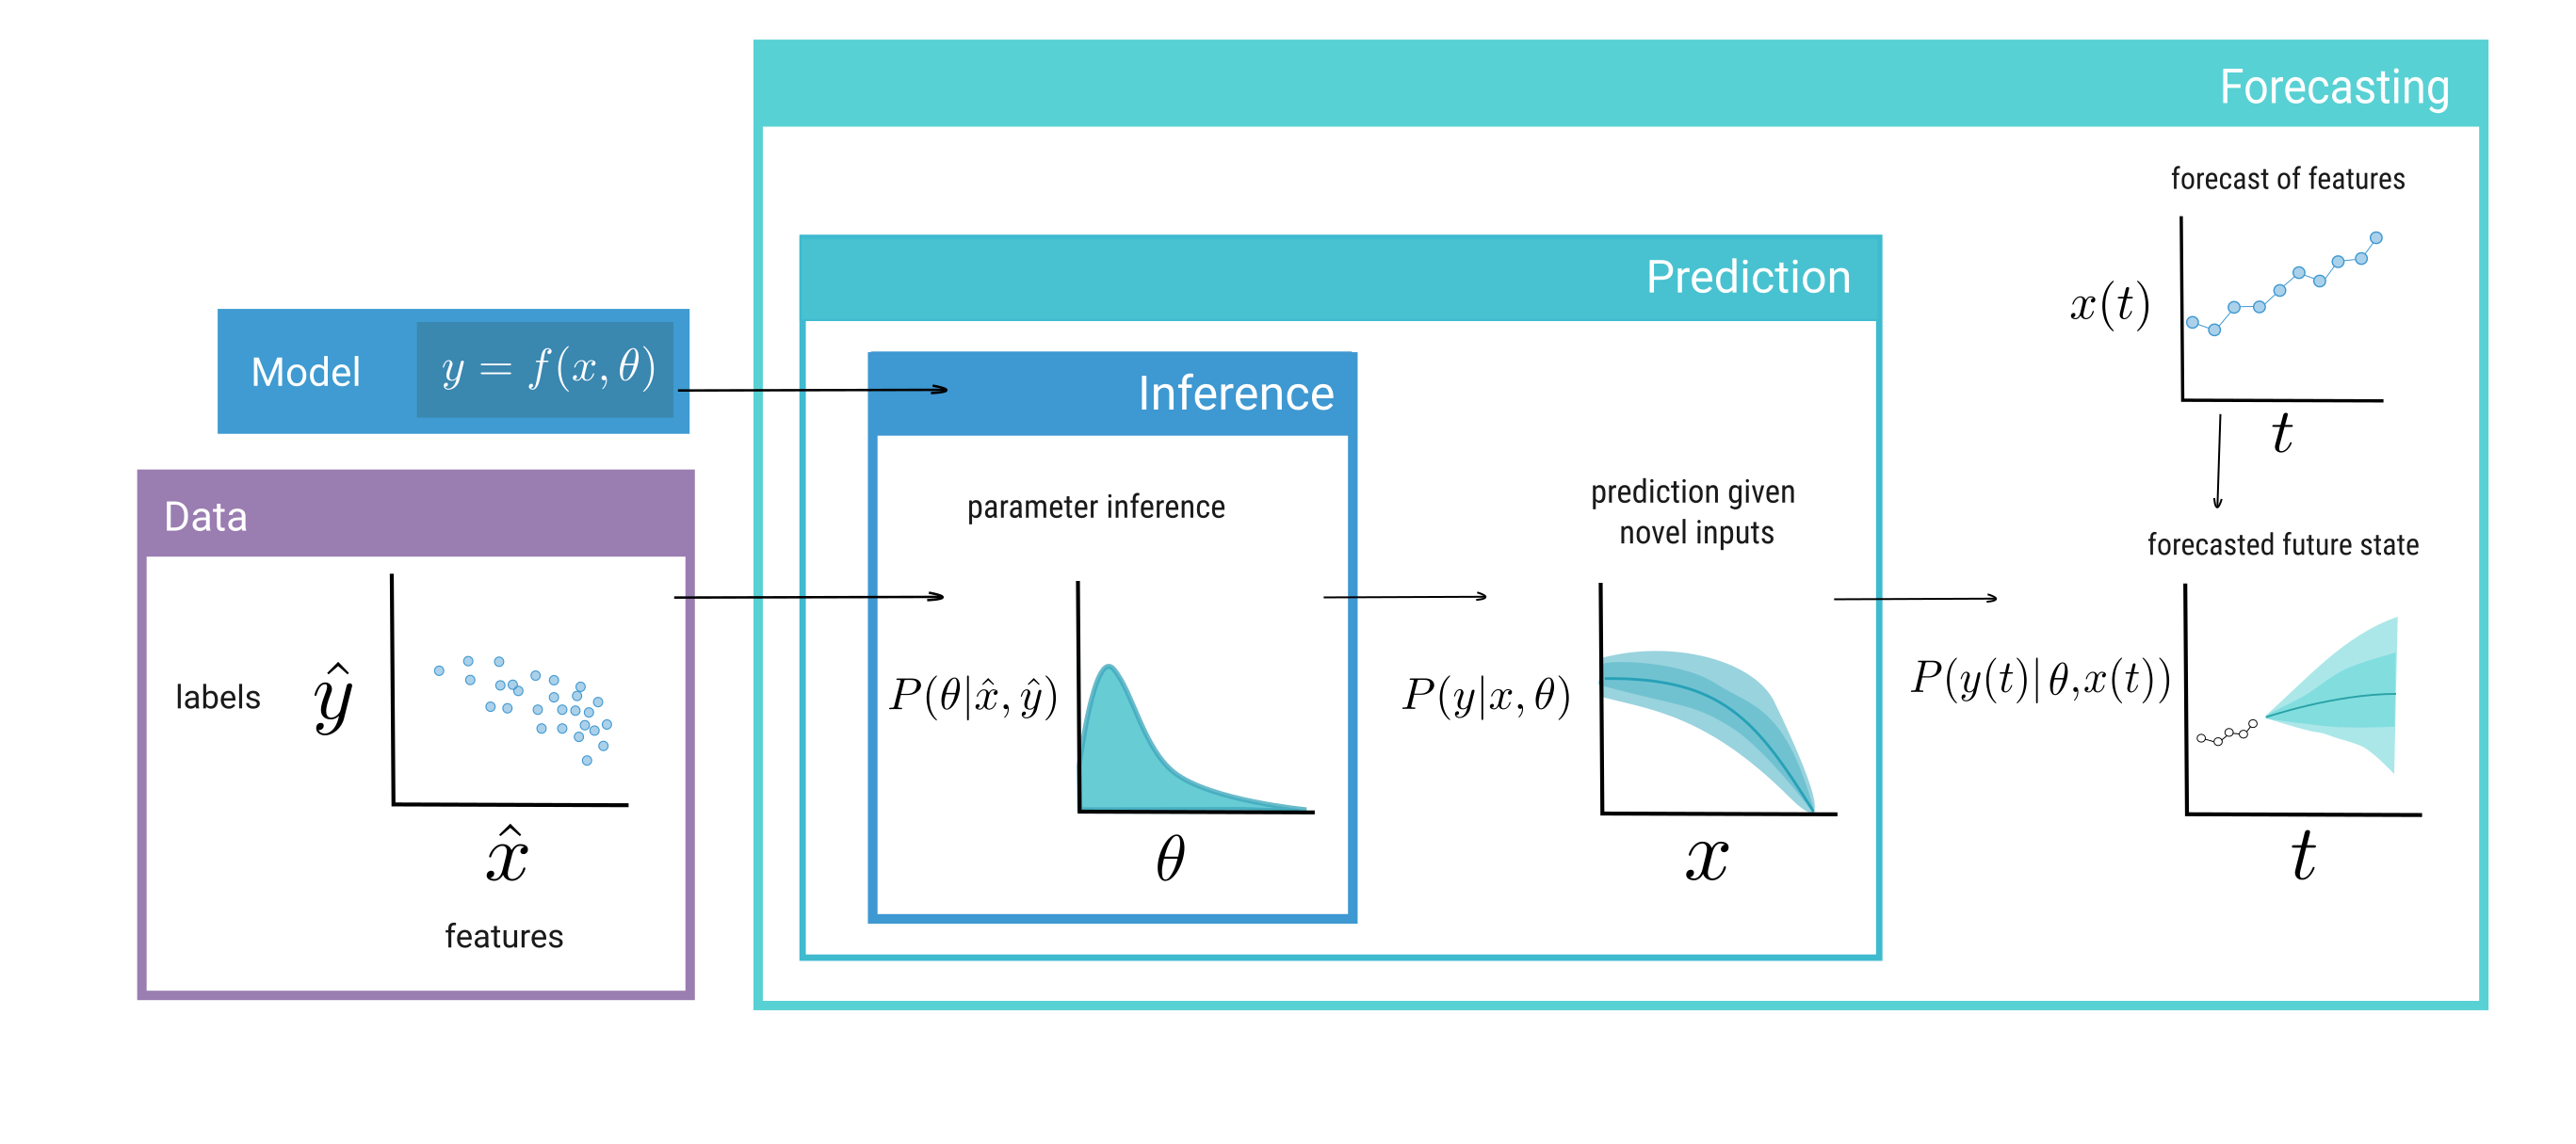
\includegraphics{figures/forecasting_v4.png}
\caption{The nested nature of developing predictive and forecasting
models, showcases the \emph{forward problem} and how this relies on a
hierarchical structure of the modelling process. The choice of a
specific modelling technique and framework, as well as the data retained
to be part of this model, proceeds directly from our assumptions about
which ecological mechanisms are important in shaping both extant and
future data.}\label{fig:models}
}
\end{figure}

\hypertarget{what-do-you-need-to-build-a-predictive-model}{%
\subsubsection{What do you need to build a predictive
model?}\label{what-do-you-need-to-build-a-predictive-model}}

To build a predictive model, one needs the following: first,
\textbf{data}, split into features \(\hat{x}\) and labels \(\hat{y}\)
(fig.~\ref{fig:models}). Second, a \textbf{model} \(f\), which maps
features \(x\) to labels \(y\) as a function of parameters \(\theta\),
i.e.~\(y = f(x, \theta)\). Third, a \textbf{loss function}
\(L(\hat{y}, y)\), which describes how far a model's prediction \(y\) is
from an empirical value \(\hat{y}\). Lastly, \textbf{priors} on
parameters, \(P(\theta)\), which describe the modeller's \emph{a priori}
belief about the value of the parameters; rather than making an analysis
implicit, specifying priors has the merit of making the modeller's
assumptions explicit, which is a most desirable feature when
communicating predictions to stakeholders (Spiegelhalter et al. 2000).
Often an important step before fitting a model is feature engineering:
adjusting and reworking the features to better uncover feature-label
relationships (Kuhn and Johnson 2019). This can include projecting the
features into a lower dimensional space, as we did through a
probabilistic PCA in the case study, or removing the covariance
structure using a Whitening approach. Then, when a model is fitted
(synonymous with parameter inference or the inverse problem, see
fig.~\ref{fig:models}), a fitting algorithm attempts to estimate the
values of \(\theta\) that minimises the mean value of loss function
\(L(\hat{y},y)\) for all labels \(\hat{y}\) in the provided data \(Y\).
In a Bayesian approach, this typically relys on drawing candidate
parameter values from priors and applying some form of sampling to
generate a posterior estimate of parameters,
\(P(\theta | \hat{x}, \hat{y})\). In the training of neural networks,
this usually involves some form of error back-propagation across the
edges in order to tune their weights, and the biases of each nodes.

\hypertarget{how-do-we-validate-a-predictive-model}{%
\subsubsection{How do we validate a predictive
model?}\label{how-do-we-validate-a-predictive-model}}

After we fit a model, we inevitably want to see how ``good'' (meaning,
``fit for purpose'') it is. This process can be divided into two parts:
(i)) model selection, where the modeller chooses from a set of possible
models and (ii) model assessment, where the modeller determines the
performance characteristics of the chosen model (Hastie, Tibshirani, and
Friedman 2009).

In the context of \emph{model selection}, a naïve initial approach is to
simply compute the average error between the model's prediction and the
true data we have, and choose the model with the smallest
error---however this approach inevitably results in \emph{overfitting}.
One approach to avoid overfitting is using information criteria (e.g.,
AIC, BIC, MDL) based around the heuristic that good models maximise the
ratio of information provided by the model to the number of parameters
it has. However, when the intended use-case of a model is prediction the
relevant form of validation is \emph{predictive accuracy}, which should
be tested with \emph{cross-validation}. Cross-validation methods divide
the original dataset into two---one which is used to fit the model
(called the \emph{training} set) and one used to validate its predictive
accuracy on the data that it hasn't ``seen'' yet (called the \emph{test}
set) (Bishop 2006). This procedure is often repeated across different
test and training subdivisions of the dataset (either picked randomly or
stratified by some criteria, like balance between positive and negative
interactions in the case study) to determine the uncertainty associated
with our measurement due to our choice of test and training sets (Arlot
and Celisse 2010), in the same conceptual vein as data bootstrapping:
the mean value of the validation metric gives an overall estimate of its
performance, and the variance around this mean represents the effect of
using different data for training and testing. In a robust model/dataset
combination, we expect this variance to be low, although there are no
prescriptive guidelines as to how little variance is acceptable; the
choice of whether to use a model is often left to the best judgement of
the modeller.

We still have to define what \emph{predictive accuracy} means in the
context of interaction network prediction. In the proof-of-concept, we
used a neural-network to perform binary classification by predicting the
presence/absence of an interaction between any two species. There are
two ways for the model to be right: the model predicts an interaction
and there is one (a \emph{true positive} (TP)), or the model predicts no
interaction and there isn't one (a \emph{true negative} (TN)).
Similarly, there are two ways for the model to be wrong: the model
predicts an interaction which does not exist (a \emph{false positive}
(FP)), or the model predicts no interaction but it does exist (a
\emph{false negative} (FN)).

A naïve initial approach to measure how well a model does is
\emph{accuracy}, i.e. the proportion of values it got correct. However,
consider what we know about interaction networks: they are often very
sparse, with connectance usually below a third (Cohen, Briand, and
Newman 1990). If we build a model that always guesses there will be no
interaction between two species, it will be correct in the majority of
cases because the majority of potential interactions in a network
typically do not exist. Therefore this ``empty-matrix'' model would
always have an \emph{accuracy} of \(1-C\), where \(C\) is the observed
connectance, which would almost always be greater than 50\%.
Understanding model performance within sensitivity-specificity space may
be more informative, where sensitivity evaluates how good the model is
at predicting true interactions (True Positive Rate) and specificity
refers to the prediction of true ``non-interactions'' (True Negative
Rate). It must be noted that in ecological networks, there is no
guarantee that the ``non-interactions'' (assumed true negatives) in the
original dataset are indeed true negatives (Jordano 2016a, 2016b). This
can result in the positive/negative values, and the false
omission/discovery being artificially worse, and specifically decrease
our confidence in predicted interactions.

In response to the general problem of biases in classifiers, many
metrics have been proposed to measure binary-classifiers (Gu, Zhu, and
Cai 2009; Drummond and Holte 2006) and are indicative of how well the
model performs with regards to some aspect of accuracy, sensitivity,
specificity and/or precision (tbl.~\ref{tbl:validation}). Ultimately the
choice of metric will depend on the intended use of the model: there is
not a single definition of ``success,'' but rather different
interpretation of what sources of error are acceptable for a given
application.

\hypertarget{tbl:validation}{}
\begin{longtable}[]{@{}llll@{}}
\caption{\label{tbl:validation}Overview of the validation statistics
applied to the case study, alongside the criteria indicating a
successful classifier and a guide to interpretation of the values. Taken
together, these validation measures indicate that the model performs
well, especially considering that it is trained from a small volume of
data.}\tabularnewline
\toprule
\begin{minipage}[b]{0.21\columnwidth}\raggedright
Name\strut
\end{minipage} & \begin{minipage}[b]{0.05\columnwidth}\raggedright
Value\strut
\end{minipage} & \begin{minipage}[b]{0.13\columnwidth}\raggedright
Success\strut
\end{minipage} & \begin{minipage}[b]{0.49\columnwidth}\raggedright
Description\strut
\end{minipage}\tabularnewline
\midrule
\endfirsthead
\toprule
\begin{minipage}[b]{0.21\columnwidth}\raggedright
Name\strut
\end{minipage} & \begin{minipage}[b]{0.05\columnwidth}\raggedright
Value\strut
\end{minipage} & \begin{minipage}[b]{0.13\columnwidth}\raggedright
Success\strut
\end{minipage} & \begin{minipage}[b]{0.49\columnwidth}\raggedright
Description\strut
\end{minipage}\tabularnewline
\midrule
\endhead
\begin{minipage}[t]{0.21\columnwidth}\raggedright
Random accuracy\strut
\end{minipage} & \begin{minipage}[t]{0.05\columnwidth}\raggedright
0.56\strut
\end{minipage} & \begin{minipage}[t]{0.13\columnwidth}\raggedright
\strut
\end{minipage} & \begin{minipage}[t]{0.49\columnwidth}\raggedright
Fraction of correct predictions if the classifier is random\strut
\end{minipage}\tabularnewline
\begin{minipage}[t]{0.21\columnwidth}\raggedright
Accuracy\strut
\end{minipage} & \begin{minipage}[t]{0.05\columnwidth}\raggedright
0.81\strut
\end{minipage} & \begin{minipage}[t]{0.13\columnwidth}\raggedright
\(\rightarrow 1\)\strut
\end{minipage} & \begin{minipage}[t]{0.49\columnwidth}\raggedright
Observed fraction of correct predictions\strut
\end{minipage}\tabularnewline
\begin{minipage}[t]{0.21\columnwidth}\raggedright
Balanced accuracy\strut
\end{minipage} & \begin{minipage}[t]{0.05\columnwidth}\raggedright
0.80\strut
\end{minipage} & \begin{minipage}[t]{0.13\columnwidth}\raggedright
\(\rightarrow 1\)\strut
\end{minipage} & \begin{minipage}[t]{0.49\columnwidth}\raggedright
Average fraction of correct positive and negative predictions\strut
\end{minipage}\tabularnewline
\begin{minipage}[t]{0.21\columnwidth}\raggedright
\strut
\end{minipage} & \begin{minipage}[t]{0.05\columnwidth}\raggedright
\strut
\end{minipage} & \begin{minipage}[t]{0.13\columnwidth}\raggedright
\strut
\end{minipage} & \begin{minipage}[t]{0.49\columnwidth}\raggedright
\strut
\end{minipage}\tabularnewline
\begin{minipage}[t]{0.21\columnwidth}\raggedright
True Positive Rate\strut
\end{minipage} & \begin{minipage}[t]{0.05\columnwidth}\raggedright
0.77\strut
\end{minipage} & \begin{minipage}[t]{0.13\columnwidth}\raggedright
\(\rightarrow 1\)\strut
\end{minipage} & \begin{minipage}[t]{0.49\columnwidth}\raggedright
Fraction of interactions predicted\strut
\end{minipage}\tabularnewline
\begin{minipage}[t]{0.21\columnwidth}\raggedright
True Negative Rate\strut
\end{minipage} & \begin{minipage}[t]{0.05\columnwidth}\raggedright
0.83\strut
\end{minipage} & \begin{minipage}[t]{0.13\columnwidth}\raggedright
\(\rightarrow 1\)\strut
\end{minipage} & \begin{minipage}[t]{0.49\columnwidth}\raggedright
Fraction of non-interactions predicted\strut
\end{minipage}\tabularnewline
\begin{minipage}[t]{0.21\columnwidth}\raggedright
False Positive Rate\strut
\end{minipage} & \begin{minipage}[t]{0.05\columnwidth}\raggedright
0.16\strut
\end{minipage} & \begin{minipage}[t]{0.13\columnwidth}\raggedright
\(\rightarrow 0\)\strut
\end{minipage} & \begin{minipage}[t]{0.49\columnwidth}\raggedright
Fraction of non-interactions predicted as interactions\strut
\end{minipage}\tabularnewline
\begin{minipage}[t]{0.21\columnwidth}\raggedright
False Negative Rate\strut
\end{minipage} & \begin{minipage}[t]{0.05\columnwidth}\raggedright
0.22\strut
\end{minipage} & \begin{minipage}[t]{0.13\columnwidth}\raggedright
\(\rightarrow 0\)\strut
\end{minipage} & \begin{minipage}[t]{0.49\columnwidth}\raggedright
Fraction of interactions predicted as non-interactions\strut
\end{minipage}\tabularnewline
\begin{minipage}[t]{0.21\columnwidth}\raggedright
\strut
\end{minipage} & \begin{minipage}[t]{0.05\columnwidth}\raggedright
\strut
\end{minipage} & \begin{minipage}[t]{0.13\columnwidth}\raggedright
\strut
\end{minipage} & \begin{minipage}[t]{0.49\columnwidth}\raggedright
\strut
\end{minipage}\tabularnewline
\begin{minipage}[t]{0.21\columnwidth}\raggedright
ROC-AUC\strut
\end{minipage} & \begin{minipage}[t]{0.05\columnwidth}\raggedright
0.86\strut
\end{minipage} & \begin{minipage}[t]{0.13\columnwidth}\raggedright
\(\rightarrow 1\)\strut
\end{minipage} & \begin{minipage}[t]{0.49\columnwidth}\raggedright
Proximity to a perfect prediction (ROC-AUC=1)\strut
\end{minipage}\tabularnewline
\begin{minipage}[t]{0.21\columnwidth}\raggedright
Youden's J\strut
\end{minipage} & \begin{minipage}[t]{0.05\columnwidth}\raggedright
0.60\strut
\end{minipage} & \begin{minipage}[t]{0.13\columnwidth}\raggedright
\(\rightarrow 1\)\strut
\end{minipage} & \begin{minipage}[t]{0.49\columnwidth}\raggedright
Informedness of predictions (trust in individual prediction)\strut
\end{minipage}\tabularnewline
\begin{minipage}[t]{0.21\columnwidth}\raggedright
Cohen's \(\kappa\)\strut
\end{minipage} & \begin{minipage}[t]{0.05\columnwidth}\raggedright
0.58\strut
\end{minipage} & \begin{minipage}[t]{0.13\columnwidth}\raggedright
\(\ge 0.5\)\strut
\end{minipage} & \begin{minipage}[t]{0.49\columnwidth}\raggedright
\strut
\end{minipage}\tabularnewline
\begin{minipage}[t]{0.21\columnwidth}\raggedright
\strut
\end{minipage} & \begin{minipage}[t]{0.05\columnwidth}\raggedright
\strut
\end{minipage} & \begin{minipage}[t]{0.13\columnwidth}\raggedright
\strut
\end{minipage} & \begin{minipage}[t]{0.49\columnwidth}\raggedright
\strut
\end{minipage}\tabularnewline
\begin{minipage}[t]{0.21\columnwidth}\raggedright
Positive Predictive Value\strut
\end{minipage} & \begin{minipage}[t]{0.05\columnwidth}\raggedright
0.66\strut
\end{minipage} & \begin{minipage}[t]{0.13\columnwidth}\raggedright
\(\rightarrow 1\)\strut
\end{minipage} & \begin{minipage}[t]{0.49\columnwidth}\raggedright
Confidence in predicted interactions\strut
\end{minipage}\tabularnewline
\begin{minipage}[t]{0.21\columnwidth}\raggedright
Negative Predictive Value\strut
\end{minipage} & \begin{minipage}[t]{0.05\columnwidth}\raggedright
0.89\strut
\end{minipage} & \begin{minipage}[t]{0.13\columnwidth}\raggedright
\(\rightarrow 1\)\strut
\end{minipage} & \begin{minipage}[t]{0.49\columnwidth}\raggedright
Confidence in predicted non-interactions\strut
\end{minipage}\tabularnewline
\begin{minipage}[t]{0.21\columnwidth}\raggedright
False Omission Rate\strut
\end{minipage} & \begin{minipage}[t]{0.05\columnwidth}\raggedright
0.10\strut
\end{minipage} & \begin{minipage}[t]{0.13\columnwidth}\raggedright
\(\rightarrow 0\)\strut
\end{minipage} & \begin{minipage}[t]{0.49\columnwidth}\raggedright
Expected proportion of missed interactions\strut
\end{minipage}\tabularnewline
\begin{minipage}[t]{0.21\columnwidth}\raggedright
False Discovery Rate\strut
\end{minipage} & \begin{minipage}[t]{0.05\columnwidth}\raggedright
0.33\strut
\end{minipage} & \begin{minipage}[t]{0.13\columnwidth}\raggedright
\(\rightarrow 0\)\strut
\end{minipage} & \begin{minipage}[t]{0.49\columnwidth}\raggedright
Expected proportion of wrongly imputed interactions\strut
\end{minipage}\tabularnewline
\bottomrule
\end{longtable}

In the machine learning literature, a common way of visualising this
extensive list of possible metrics is through the use of ROC
(receiver-operating-characteristic; False Positive Rate on the x-axis,
and True Positive Rate on the y-axis) and PR (precision-recall;
True-Positive-Rate on the x-axis, Positive-predictive-value on the
y-axis) curves (see fig.~\ref{fig:example}). These curves are generated
by considering a continuum of thresholds of classifier acceptance, and
computing the values of ROC/PR metrics for each value of the threshold.
The area-under-the-curve (AUC) is then used as a validation metric and
are typically called AUC-ROC (Area-Under-the-Curve
Receiver-Operator-Curve) and AUC-PR (Area-Under-the-Curve
Precision-Recall) (e.g.~ROC-AUC in tbl.~\ref{tbl:validation}). These
measures have the unstated assumption that the training and testing set
are ``correct,'' or at least correct enough that the number of
true/false positive/negatives are meaningful; although should this
assumption be true, there would be no need for any predictive approach
-- but it is a well established fact that machine learning systems are
resilient to even relatively high uncertainties in the data (Halevy,
Norvig, and Pereira 2009).

\hypertarget{networks-and-interactions-as-predictable-objects}{%
\subsection{Networks and interactions as predictable
objects}\label{networks-and-interactions-as-predictable-objects}}

\hypertarget{why-predict-networks-and-interactions-at-the-same-time}{%
\subsubsection{Why predict networks and interactions at the same
time?}\label{why-predict-networks-and-interactions-at-the-same-time}}

Ecological networks are quite sparse, and larger networks tend to get
sparser (MacDonald, Banville, and Poisot 2020); in other words, although
networks are composed of a set of interactions between species pairs,
they also form a much larger set of species pairs that do not interact.
If we aim to predict the structure of networks from the ``bottom-up''---
by considering each pairwise combination of \(S\) different species---we
are left with \(S^2\) interaction values to estimate, a majority of
which will be 0. Instead, we can use our existing understanding of the
mechanisms that structure ecological networks to whittle down the set of
feasible adjacency matrices, thereby reducing the amount of information
we must predict, and making the problem of predicting interactions less
daunting. The processes that structure ecological networks do not only
occur at the scale of interactions---there are also processes at the
network level which limit what interactions (or how many) are realistic.
The realised structure of a network is the synthesis of the interactions
forming the basis for network structure, and the network structure
refining the possible interactions---``Part makes whole, and whole makes
part'' (Levins and Lewontin 1987).

Another argument for the joint prediction of networks and interactions
is to reduce circularity and biases in the predictions. As an example,
models like linear filtering (Stock et al. 2017) generate probabilities
of non-observed interactions existing, but do so based on measured
network properties. Some recent models make interaction-level
predictions (e.g. Gravel et al. 2019); these are not unlike stacked
species distribution models, which are individually fit, but
collectively outperformed by joint models or rule-based models (Zurell
et al. 2020). By relying on adequate testing of model performance of
biases (i.e.~optimising not only accuracy, but paying attention to
measures like false discovery and false omission rates), and developing
models around a feedback loop between network and interaction
prediction, it is likely that the quality of the predicted networks will
be greatly improved compared to current models.

\hypertarget{what-network-properties-should-we-use-to-inform-our-predictions-of-interactions}{%
\subsubsection{What network properties should we use to inform our
predictions of
interactions?}\label{what-network-properties-should-we-use-to-inform-our-predictions-of-interactions}}

There are many dimensions of network structure (Delmas et al. 2018), yet
there are two arguments to support basing network prediction around a
single property: \emph{connectance} (the ratio of actual edges to
possible edges in the network). First, connectance is ecologically
informative---it relates to resilience to invasion (Baiser, Russell, and
Lockwood 2010; Smith-Ramesh, Moore, and Schmitz 2016), can increase
robustness to extinction in food webs (J. Dunne, Williams, and Martinez
2002), while decreasing it in mutualistic networks (Vieira and
Almeida-Neto 2015), and connectance relates to network stability (Landi
et al. 2018). Second, most (if not all) network properties covary with
connectance (Poisot and Gravel 2014; J. A. Dunne, Williams, and Martinez
2002).

Within the network science literature, there are numerous methods for
predicting edges based on network properties (e.g., block models (Yen
and Larremore 2020) based on modularity, hierarchical models (Kawakatsu
et al. 2021) based on embedding, etc.). However, in the context of
species interaction networks, these properties often covary with
connectance. As a result we suggest that using connectance as the
primary property of interest is most likely to be practical to formulate
at the moment. We have models to estimate species richness over space
(Jenkins, Pimm, and Joppa 2013), and because we can predict connectance
from species richness alone (MacDonald, Banville, and Poisot 2020), we
can then derive distributions of network properties from richness
estimates, that can serve to penalise further models that formulate
their predictions at the scale of each possible interaction.

\hypertarget{how-do-we-predict-how-species-that-we-have-never-observed-together-will-interact}{%
\subsubsection{How do we predict how species that we have never observed
together will
interact?}\label{how-do-we-predict-how-species-that-we-have-never-observed-together-will-interact}}

A neutral approach to ecological interactions would assume the
probability of an interaction to mirror the relative abundance of both
species, and would be unaffected by trait variation (Poisot, Stouffer,
and Gravel 2015; Pichler et al. 2020); more accurately, a neutral
assumption states that the relative abundances are sufficient to predict
the structure of networks, and this view is rather well supported in
empirical and theoretical systems (Canard et al. 2012, 2014). However,
functional-trait based proxies could enable better predictions of
ecological interactions (Cirtwill and Eklöf 2018; Cirtwill et al. 2019;
Bartomeus et al. 2016; Bartomeus 2013). Selection on functional traits
could cause interactions to be conserved at some evolutionary scales,
and therefore predictions of interaction could be informed by
phylogenetic analyses (Davies 2021; Elmasri et al. 2020; Gómez, Verdú,
and Perfectti 2010). Phylogenetic matching in bipartite networks is
consistent across scales (Poisot and Stouffer 2018), even in the absence
of strong selective pressure (Coelho, Rodrigues, and Rangel 2017).

A separate family of methods are based on network embedding (as in the
proof-of-concept). A network embedding projects each node of the network
into a lower-dimensional latent space. Previous explorations of the
dimensionality of food webs have revealed that a reduced number of
dimensions (7) was sufficient to capture most of their structure (Eklöf
et al. 2013); however, recent quantifications of the complexity of the
embedding space of bipartite ecological networks found a consistent high
complexity (Strydom, Dalla Riva, and Poisot 2021), suggesting that the
precise depth of embedding required may vary considerably across
systems. Embeddings enables us to represent the structure of a network,
which previously required the \(S^2\) dimensions of an adjacency matrix,
with a smaller number of dimensions. The position of each node in this
lower dimensional space is then treated as a latent measurement
corresponding to the role of that species in the network (e.g. Poisot,
Ouellet, et al. 2021, where a network of about 1500 species was most
accurately described using 12 dimensions). Species close together in the
latent space should interact with similar set of species (Rossberg et
al. 2006; Rohr et al. 2010). However, these models are sensitive to
sampling biases as they are limited to species for which there is
already interaction data, and as a result a methodological breakthrough
is needed to extend these models to species for which there is little or
no interaction data.

\hypertarget{how-do-we-quantify-interaction-strength}{%
\subsubsection{How do we quantify interaction
strength?}\label{how-do-we-quantify-interaction-strength}}

Species interaction networks can also be used as a means to quantify and
understand \emph{interaction strength}. Interaction strength, unlike the
qualitative presence or absence of an interaction, is a continuous
measurement which attempts to quantify the effect of one species on
another. This results in weighted networks representing different
patterns of `flows' between nodes -- which can be modelled in a variety
of ways (Borrett and Scharler 2019). Interaction strength can generally
be divided into two main categories (as suggested by Berlow et al.
(2004)): 1) the strength of an interaction between individuals of each
species, or 2) the effect that changes in one species population has on
the dynamics of the other species. It can be measured as the effect over
a period of time (in the units of biomass or energy flux (Barnes et al.
2018; Brown et al. 2004)) or the relative importance of one species on
another (Heleno et al. 2014; Berlow et al. 2004; Wootton and Emmerson
2005). One recurring observation is that networks are often composed of
many weak interactions and few strong interactions (Berlow et al. 2004).
The distribution of interaction strength within a network effects its
stability (Neutel 2002; Ruiter, Neutel, and Moore 1995) and functioning
(Duffy 2002; José M. Montoya, Rodríguez, and Hawkins 2003), and serves
to benefit multi-species models (Wootton and Emmerson 2005).
Alternatively, understanding flow in modules within networks can aid in
understanding the organisation of networks (Farage et al. 2021; Jose M.
Montoya and Solé 2002) or the cascading effects of perturbations
(Gaiarsa and Guimarães 2019).

In some systems, quantifying interaction strength is relatively
straightforward; this includes a lot of host-parasite systems. For
example, freshwater cyprinid fish can be divided in micro-habitats
(fins, skin, digestive system, gill subsections) and the parasites
counted in each of these micro-habitats, giving within-host resolution
(Simková et al. 2002); marine sparids and labrids have similarly been
studied this way, see notably (Sasal, Niquil, and Bartoli 1999;
Desdevises 2006; Morand et al. 2002). In some cases, within-host
assessments of interaction strengths can reveal macro-ecological events,
like in the conservatism of micro-habitat use in amphibian hosts by
helminths (Badets et al. 2011). Even ectoparasites can provide reliable
assessments of interaction strength; for example, when rodent hosts are
minimally disturbed during capture, fine combing of their fur will
result in exhaustive ectoparasites inventories (Hadfield et al. 2014;
Karbowiak et al. 2019; Matthee et al. 2020; Sánchez et al. 2014; E. R.
Dickinson, Millins, and Biek 2020). Parasites have the desirable
property of usually remaining intact within their host during the
interaction, as opposed to prey items as can be recovered through
\emph{e.g.} gut content analysis or stable isotopes (Macías-Hernández et
al. 2018; Schmid-Araya et al. 2016). As network ecology is starting to
explore the use of predictive models, leading up to forecasting, we
argue that host-parasite systems can provide data that are reliable and
trustworthy enough that they can become the foundations for
methodological development and benchmark studies, thereby providing more
information about host-parasite systems and supporting the technical
development of the field.

Yet in most situations, much like quantifying the occurrence of an
interaction, quantifying interaction \emph{strength} in the field is
challenging in the majority of systems, and one must often rely on
proxies. In some contexts, interaction strength can be estimated via
functional foraging (Portalier et al. 2019), where the primary basis for
inferring interaction is foraging behaviour like searching, capture and
handling times. In food-webs, metabolic based models use body mass,
metabolic demands, and energy loss to infer energy fluxes between
organisms (Yodzis and Innes 1992; Berlow et al. 2009). In addition,
food-web energetics models can be incorporated at various resolutions
for a specific network, ranging from individual-based data to more
lumped data at the species level or trophic group, depending on data
availability (Barnes et al. 2018; Berlow et al. 2009). Taken together,
these considerations impose too many constraints on predicting
continuous interaction strength at the moment, resulting in our primary
focus in binary present/absent interactions within this manuscript.

\hypertarget{how-do-we-determine-what-interaction-networks-are-feasible}{%
\subsubsection{How do we determine what interaction networks are
feasible?}\label{how-do-we-determine-what-interaction-networks-are-feasible}}

For several decades, ecologists have aimed to understand how networks of
many interacting species persist through time. The diversity-stability
paradox, first explored by May (1974), shows that under a neutral set of
assumptions ecological networks should become decreasingly stable as the
number of species increases. Yet, in the natural world we observe
networks of interactions that consist of far more species than May's
model predicts (Albouy et al. 2019). As a result, understanding what
aspects of the neutral assumptions of May's model are incorrect has
branched many investigations into the relationship between ecological
network structure and persistence (Allesina and Tang 2012). These
assumptions can be split into dynamical assumptions and topological
assumptions. Topologically, we know that ecological networks are not
structured randomly. Some properties, like the aforementioned
connectance, are highly predictable (MacDonald, Banville, and Poisot
2020). Generative models of food-webs (based on network embeddings) fit
empirical networks more effectively than random models (Allesina,
Alonso, and Pascual 2008). These models have long used allometry as a
single-dimensional niche space---naturally we want to extend this to
traits in general. The second approach to stability is through
\emph{dynamics}. Early models of community dynamics rely on the
assumption of linear interaction effects, but in recent years models of
bioenergetic community dynamics have shown promise in basing our
understanding of energy flow in food-webs in the understood relationship
between allometry and metabolism (Delmas et al. 2017). An additional
consideration is the multidimensional nature of ``stability'' and
``feasibility'' (e.g.~resilience to environmental change vs extinctions)
(Domínguez-García, Dakos, and Kéfi 2019) and how different disturbances
propagate across levels of biological organisation (Kéfi et al. 2019;
Gravel, Massol, and Leibold 2016). Recent approaches such as structural
stability (Saavedra et al. 2017; Ferrera, Pascual-García, and Bastolla
2016) allow us to think of network feasibility in rigorous mathematical
terms, which may end up as usable parameters to penalise network
predictions.

\hypertarget{what-taxonomic-scales-are-suitable-for-the-prediction-of-species-interactions}{%
\subsubsection{What taxonomic scales are suitable for the prediction of
species
interactions?}\label{what-taxonomic-scales-are-suitable-for-the-prediction-of-species-interactions}}

If we use different trait-based proxies to predict potential
interactions between species the choice of such proxies should be
theoretically linked to the taxonomic and spatial scale we are using in
our prediction (Wiens 1989). At some scales we can use morphological
traits of co-occurring species to assess the probability of interaction
between them (Bartomeus et al. 2016). On broader taxonomic scales we can
infer interaction probability through the phylogenetic distance,
assuming that functional traits themselves are conserved (Gómez, Verdú,
and Perfectti 2010). In this case, we can think of the probability that
one species will interact with another as the distance between them in
niche-space (Desjardins-Proulx et al. 2017), and this can be modelled by
simulating neutral expectations of trait variation on phylogenetic trees
(Davies 2021). At the narrowest scales, we may be interested in
predicting behavioural traits like foraging behaviour (Bartomeus et al.
2016), and at this scale we may need to consider abundance's effect on
the probability of an encounter (Wells and O'Hara 2013).

\hypertarget{what-about-indirect-and-higher-order-interactions}{%
\subsubsection{What about indirect and higher-order
interactions?}\label{what-about-indirect-and-higher-order-interactions}}

Although network ecology often assumes that interactions go strictly
from one node to the other, the web of life is made up of a variety of
interactions. Indirect interactions---either higher-order interactions
between species, or interaction strengths that themselves interact ---
have gained interest in recent years (Golubski et al. 2016; Golubski and
Abrams 2011). One mathematical tool to describe these situations is
hypergraphs: hypergraphs are the generalisation of a graph, allowing a
broad yet manageable approach to complex interactions (Carletti,
Fanelli, and Nicoletti 2020), by allowing for particular interactions to
occur beyond a pair of nodes. An additional degree of complexity is
introduced by multi-layer networks (Hutchinson et al. 2019). Multi-layer
networks include edges across ``variants'' of the networks (timepoints,
locations, or environments). These can be particularly useful to account
for the metacommunity structure (Gross et al. 2020), or to understand
how dispersal can inform conservation action (Albert et al. 2017).
Ecological networks are intrinsically multi-layered (Pilosof et al.
2017). However, \emph{prima facie}, increasing the dimensionality of the
object we need to predict (the multiple layers rather than a single
network) makes the problem more complicated. Yet, multi-layer approaches
improve prediction in social networks (Jalili et al. 2017; Najari et al.
2019; Yasami and Safaei 2018), and they may prove useful in network
ecology going forward.

\hypertarget{space}{%
\subsection{Space}\label{space}}

Although networks were initially used to describe the interactions
\emph{within} a community, interest in the last decade has shifted
towards understanding their structure and variation over space
(Trøjelsgaard and Olesen 2016; Baiser et al. 2019), and has established
network ecology as an important emerging component of biogeography and
macroecology.

\hypertarget{how-much-do-networks-vary-over-space}{%
\subsubsection{How much do networks vary over
space?}\label{how-much-do-networks-vary-over-space}}

Networks can vary across space either in their structural properties
(e.g. connectance or degree distribution) or in their composition
(identity of nodes and edges). Interestingly, variation in the
structural properties of ecological networks primarily responds to
changes in the size of the network. The number of links in ecological
networks scales with the number of species (MacDonald, Banville, and
Poisot 2020; Brose et al. 2004), and connectance and size drive the rest
of network structure (Poisot and Gravel 2014; J. A. Dunne, Williams, and
Martinez 2002; Riede et al. 2010). Species turnover in space results in
changes in the composition of ecological networks. But, this is not the
only reason network composition varies (Poisot, Stouffer, and Gravel
2015). Intraspecific variation can result in interaction turnovers
without changes in species composition (Bolnick et al. 2011). Similarly,
changes in species abundances can lead to variation in interaction
strengths (Canard et al. 2014; Vázquez et al. 2007). Variation in the
abiotic environment and indirect interactions (Golubski et al. 2016)
could modify the occurrence and strength of individual interactions.
Despite this, empirical networks tend to share a common backbone (Mora
et al. 2018) and functional composition (Dehling et al. 2020) across
space.

\hypertarget{how-do-we-predict-what-the-species-pool-at-a-particular-location-is}{%
\subsubsection{How do we predict what the species pool at a particular
location
is?}\label{how-do-we-predict-what-the-species-pool-at-a-particular-location-is}}

As the species pool forms the basis for network structure, predicting
which species are present at a particular location is essential to
predict networks across space. Species distribution models (SDMs) are
increasingly ubiquitous in macroecology--- these models predict the
range of a species based on known occurrences and environmental
conditions, such as climate and land cover (Guisan and Thuiller 2005;
Elith et al. 2006). Including interactions or co-occurrences in SDMs
generally improves predictive performance (Wisz et al. 2013). Several
approaches exist to combine multiple SDMs: community assemblage at a
particular site can be predicted either by combining independent
single-species SDMs (stacked-SDMs, SSDMs) or by directly modelling the
entire species assemblage and multiple species at the same time (joint
SDMs, JSDMs) (Norberg et al. 2019). Building on the JSDM framework,
hierarchical modelling of species communities (Ovaskainen et al. 2017)
has the advantage of capturing processes that structure communities.
Spatially Explicit Species Assemblage Modelling (SESAM) constrains SDM
predictions using macro-ecological models (Guisan and Rahbek 2011) ---
for example, variation in species richness across space can constrain
assemblage predictions (D'Amen et al. 2015).

The next step is to constrain distribution predictions using network
properties. This builds on previous calls to adopt a probabilistic view:
a probabilistic species pool (Karger et al. 2016), and probabilistic
interactions through Bayesian networks (Staniczenko et al. 2017).
Blanchet, Cazelles, and Gravel (2020) argue that the probabilistic view
avoids confusion between interactions and co-occurrences, but that it
requires prior knowledge of interactions. This could potentially be
solved through our framework of predicting networks first, interactions
next, and finally the realised species pool.

\hypertarget{how-do-we-combine-spatial-and-network-predictions}{%
\subsubsection{How do we combine spatial and network
predictions?}\label{how-do-we-combine-spatial-and-network-predictions}}

In order to predict networks across space, we need to combine multiple
models---one which predicts what the species pool will be at a given
location, and one to predict what interaction networks composed from
this species pool are likely to be (see fig.~\ref{fig:conceptual}). Both
of these models contain uncertainty, and when we combine them the
uncertainty from each model should be propagated into the combined
model. The Bayesian paradigm provides a convenient solution to this---if
we have a chain of models where each model feeds into the next, we can
sample from the posterior of the input models. A different approach is
\emph{ensemble modelling} which combines the predictions made by several
models, where each model is predicting the same thing (Parker 2013).
Error propagation, an important step in building any ecological model,
describes the effect of the uncertainty of input variables on the
uncertainty of output variables (Draper 1995; Parysow, Gertner, and
Westervelt 2000). Benke et al. (2018) identifies two broad approaches to
model error propagation: analytically using differential equations or
stochastically using Monte-Carlo simulation methods. Errors induced by
the spatial or temporal extrapolation of data also need to be taken into
account when estimating the uncertainty of a model's output (Peters and
Herrick 2004).

\hypertarget{time}{%
\subsection{Time}\label{time}}

\hypertarget{why-should-we-forecast-species-interaction-networks}{%
\subsubsection{Why should we forecast species interaction
networks?}\label{why-should-we-forecast-species-interaction-networks}}

Forecasting species interactions are critical for informing ecosystem
management (Harvey et al. 2017) and systematic conservation
prioritisation (Pollock et al. 2020), and for anticipating extinctions
and their consequences (McDonald-Madden et al. 2016; McWilliams et al.
2019). Ecological interactions shape species distributions at both local
and broad spatial scales, and including interactions in SDM models
typically improves predictive performance (M. B. Araújo and Luoto 2007;
Wisz et al. 2013; Pigot and Tobias 2013). However, these tend to rely on
approaches involving estimating pairwise dependencies based on
co-occurrence, using surrogates for biotic-interaction gradients, and
hybridising SDMs with dynamic models (Wisz et al. 2013). Most existing
models to predict the future distribution of species ignore interactions
(Urban et al. 2016). Changes in species ranges and phenology will
inevitably create spatiotemporal mismatches and affect encounter rates
between species (Gilman et al. 2010), which will further shift the
distribution of species across space. New interactions will also appear
between species that are not currently co-occurring (Gilman et al.
2010). Only by forecasting how species will interact can we hope to have
an accurate portrait of how biodiversity will be distributed under the
future climate.

Forecasting how climate change will alter biodiversity is also crucial
for maximising conservation outcomes. Improving SDMs through
interactions is crucial for conservation, as nearly 30\% of models in
SDM studies are used to assess population declines or landscape ability
to support populations (M. B. Araújo et al. 2019). Reliable predictions
about how ecological networks will change over time will give us
critical information that could be communicated to decision-makers and
the scientific community about what future environmental risks we are
awaiting and how to mitigate them (Kindsvater et al. 2018). Not only
this, but how biodiversity is structured influences the functioning of
the whole ecosystem, community stability and persistence (Thompson et
al. 2012; Stouffer and Bascompte 2010). Will climate change impact the
distribution of network properties (e.g.~connectance)? If so, which
regions or species groups need special conservation efforts? These
overarching questions are yet to be answered (but see Albouy et al.
2013; Kortsch et al. 2015; Hattab et al. 2016). We believe that the path
toward forecasting ecological networks provides useful guidelines to
ultimately better predict how climate change will affect the different
dimensions of biodiversity and ecosystem functioning.

\hypertarget{how-do-we-turn-a-predictive-model-into-a-forecasting-model}{%
\subsubsection{How do we turn a predictive model into a forecasting
model?}\label{how-do-we-turn-a-predictive-model-into-a-forecasting-model}}

On some scales, empirical time-series encode enough information about
ecological processes for machine-learning approaches to make accurate
forecasts. However, there is an intrinsic limit to the predictability of
ecological time-series (Pennekamp et al. 2019). A forecast inherently
has a \emph{resolution limit} in space, time, and organisation. For
example, one could never hope to predict the precise abundance of every
species on Earth on every day hundreds of years into the future. There
is often a trade-off between the resolution and horizon of forecast,
e.g., a lower resolution forecast, like primary production will be at a
maximum in the summer, is likely to be true much further into the future
than a higher resolution forecast. If we want to forecast the structure
of ecological networks beyond the forecasting horizon of time-series
based methods, we need forecasts of our predictive model's inputs---a
forecast of the distribution of both environmental conditions and the
potential species pool across space (fig.~\ref{fig:models}).

\hypertarget{how-can-we-validate-a-forecasting-model}{%
\subsubsection{How can we validate a forecasting
model?}\label{how-can-we-validate-a-forecasting-model}}

Often the purpose of building a forecasting model is to inform
\emph{present} action (Dietze et al. 2018). Yet, the nature of
forecasting---trying to predict the future---is that you can only know
if a forecast is ``right'' once it is too late to change it. If we want
to maximise the chance that reality falls within a forecasting model's
predictions, there are two directions to approach this problem: the
first is to extend model validation techniques to a forecasting context,
and the second is to attempt to maximise the amount of uncertainty in
the forecast without compromising its resolution. Cross-validation (see
\emph{How do we validate a predictive model?}) can be used to test the
efficacy of a forecasting model. Given a time-series of \(N\)
observations, a model can iteratively be trained on the first \(n\)
time-points of data, and the forecasting model's accuracy can be
evaluated on the remaining time-points it hasn't ``seen'' (Bishop 2006).
This enables us to understand both how much temporal data is required
for a model to be robust, and also enables us to explore the
\emph{forecasting horizon} of a process. Further, this approach can also
be applied in the opposite temporal direction--- if we have reliable
data from the past, ``hindcasting'' can also be used to test a
forecast's robustness.

However, these methods inevitably bump into a hard-limitation on what is
feasible for a forecasting model. The future is uncertain. Any empirical
time-series we use to validate a model was collected in past conditions
that may not persist into the future. Any system we wish to forecast
will undergo only one of many possible scenarios, yet we can only
observe the realised outcome of the system under the scenario that
actually unfolds. It is therefore impossible to assess the quality of a
forecasting model in scenarios that remain hypothetical. If the goal is
to maximise the probability that reality will fall within the forecast's
estimates, forecasts should incorporate as much uncertainty about the
future scenario as possible---one way to do this is ensemble modelling
(Parker 2013). However, as we increase the amount of uncertainty we
incorporate into a forecasting model, the resolution of the forecast's
predictions could shrink (Lei and Whitaker 2017), and therefore the
modeller should be mindful of the trade-off between resolution and
accuracy when developing any forecast. Finally, ensemble models are not
guaranteed to give more accurate results: for example, Becker et al.
(2020) noted that the ensemble model outperforms the best-in-class
models, which should be taken as an indication that careful model
building and selection is of the utmost importance when dealing with a
problem as complex as the prediction of species interactions.

\hypertarget{conclusion-why-should-we-predict-species-interaction-networks}{%
\section{Conclusion: why should we predict species interaction
networks?}\label{conclusion-why-should-we-predict-species-interaction-networks}}

Because we almost can, and because we definitely should.

A better understanding of species interactions, and the networks they
form, would help unify the fields of community, network, and spatial
ecology; improve the quantification of the functional relationships
between species (Dehling and Stouffer 2018; O'Connor et al. 2020);
re-evaluate metacommunities in light of network structure (Guzman et al.
2019); and enable a new line of research into the biogeography of
species interactions (Massol et al. 2017; Braga et al. 2019) which
incorporates a synthesis of both Eltonian and Grinnellian niche (Gravel
et al. 2019). Further, the ability to reliably predict and forecast
species interactions would inform conservation efforts for protecting
species, communities, and ecosystems. Integration of species
interactions into the assessment of vulnerability to climate change is a
needed methodological advancement (Foden and Young 2016). International
panels draw on models to establish scientific consensus (M. B. Araújo et
al. 2019), and they can be improved through more effective prediction of
species distributions and interactions (Syfert et al. 2014). Further,
recent studies argue for a shift in focus from species to interaction
networks for biodiversity conservation to better understand ecosystem
processes (Harvey et al. 2017).

We should invest in network prediction because the right conditions to
do so reliably and rapidly are beginning to emerge. Given the possible
benefits to a variety of ecological disciplines that would result from
an increased ability to predict networks, we feel strongly that the
research agenda we outline here should be picked up by the community.
Although novel technologies are bringing massive amounts of data to some
parts of ecology (primarily environmental DNA and remote sensing, but
now more commonly image analysis and bioacoustics), it is even more
important to be intentional about \emph{reconciling} data. This involves
not only the work of understanding the processes encoded within data,
but also the groundwork of developing pipelines to bridge the
ever-expanding gap between ``high-throughput'' and ``low-throughput''
sampling methods. An overall increase in the volume of data will not
result in an increase of our predictive capacity as long as this data
increase is limited to specific aspects of the problem. In the areas we
highlight in fig.~\ref{fig:conceptual}, many data steps are still
limiting: documenting empirical interactions is natural history work
that doesn't lend itself to systematic automation; expert knowledge is
by design a social process that may be slightly accelerated by text
mining and natural language processing (but is not yet, or not routinely
or at scale). These limitations are affecting our ability to reconstruct
networks.

But the tools to which we feed these data, incomplete as they may be,
are gradually getting better; that is, they can do predictions faster,
they handle uncertainty and propagate it well, and they can accommodate
data volumes that are lower than we may expect (Pichler et al. 2020). It
is clear attempting to predict the structure of ecological networks at
any scale is a methodological and ecological challenge; yet it will
result in qualitative changes in our understanding of complex adaptive
systems, as well as changes to our ability to leverage information about
network structure for conservation decision. It is perhaps even more
important to forecast the structure of ecological networks because it is
commonly neglected as a facet of biodiversity that can (and should) be
managed. In fact, none of the Aichi targets mention biostructure or its
protection, despite this being recognised as an important task (McCann
2007), either implicitly or explicitly. Being able to generate reliable
datasets on networks in space or time will make this information more
actionable.

\textbf{Acknowledgements:} We acknowledge that this study was conducted
on land within the traditional unceded territory of the Saint Lawrence
Iroquoian, Anishinabewaki, Mohawk, Huron-Wendat, and Omàmiwininiwak
nations. TS, NF, TP are funded by a donation from the Courtois
Foundation; FB, NF, and TP are funded by IVADO; BM is funded by the
NSERC Alexander Graham Bell Canada Graduate Scholarship and the FRQNT
master's scholarship; FB, GD, NF, and GH are funded by the NSERC
BIOS\(^2\) CREATE program; GD is funded by the FRQNT doctoral
scholarship; DC, TS, LP, and TP are funded by the Canadian Institute of
Ecology \& Evolution; this research was enabled in part by support
provided by Calcul Québec (www.calculquebec.ca) and Compute Canada
(www.computecanada.ca). This work was supported by funding to the Viral
Emergence Research Initiative (VERENA) consortium including NSF BII
2021909. AG and MDC are supported in part by the Liber Ero Chair.

\hypertarget{references}{%
\section*{References}\label{references}}
\addcontentsline{toc}{section}{References}

\hypertarget{refs}{}
\begin{CSLReferences}{1}{0}
\leavevmode\hypertarget{ref-deAguiar2019RevBia}{}%
Aguiar, Marcus A. M. de, Erica A. Newman, Mathias M. Pires, Justin D.
Yeakel, Carl Boettiger, Laura A. Burkle, Dominique Gravel, et al. 2019.
{``Revealing Biases in the Sampling of Ecological Interaction
Networks.''} \emph{PeerJ} 7 (September): e7566.
\url{https://doi.org/10.7717/peerj.7566}.

\leavevmode\hypertarget{ref-Albert2017AppNet}{}%
Albert, Cécile H., Bronwyn Rayfield, Maria Dumitru, and Andrew Gonzalez.
2017. {``Applying Network Theory to Prioritize Multispecies Habitat
Networks That Are Robust to Climate and Land-Use Change: Prioritizing a
Network for Biodiversity.''} \emph{Conservation Biology} 31 (6):
1383--96. \url{https://doi.org/10.1111/cobi.12943}.

\leavevmode\hypertarget{ref-Albouy2019MarFis}{}%
Albouy, Camille, Philippe Archambault, Ward Appeltans, Miguel B. Araújo,
David Beauchesne, Kevin Cazelles, Alyssa R. Cirtwill, et al. 2019.
{``The Marine Fish Food Web Is Globally Connected.''} \emph{Nature
Ecology \& Evolution} 3 (8): 1153--61.
\url{https://doi.org/10.1038/s41559-019-0950-y}.

\leavevmode\hypertarget{ref-Albouy2013ProCli}{}%
Albouy, Camille, François Guilhaumon, Fabien Leprieur, Frida Ben Rais
Lasram, Samuel Somot, Roland Aznar, Laure Velez, François Le Loc'h, and
David Mouillot. 2013. {``Projected Climate Change and the Changing
Biogeography of Coastal Mediterranean Fishes.''} Edited by Peter
Pearman. \emph{Journal of Biogeography} 40 (3): 534--47.
\url{https://doi.org/10.1111/jbi.12013}.

\leavevmode\hypertarget{ref-Albrecht2018PlaAni}{}%
Albrecht, Jörg, Alice Classen, Maximilian G. R. Vollstädt, Antonia Mayr,
Neduvoto P. Mollel, David Schellenberger Costa, Hamadi I. Dulle, et al.
2018. {``Plant and Animal Functional Diversity Drive Mutualistic Network
Assembly Across an Elevational Gradient.''} \emph{Nature Communications}
9 (1): 3177. \url{https://doi.org/10.1038/s41467-018-05610-w}.

\leavevmode\hypertarget{ref-Allesina2008GenMod}{}%
Allesina, Stefano, David Alonso, and Mercedes Pascual. 2008. {``A
General Model for Food Web Structure.''} \emph{Science} 320 (5876):
658--61. \url{https://doi.org/10.1126/science.1156269}.

\leavevmode\hypertarget{ref-Allesina2012StaCri}{}%
Allesina, Stefano, and Si Tang. 2012. {``Stability Criteria for Complex
Ecosystems.''} \emph{Nature} 483 (7388): 205--8.
\url{https://doi.org/10.1038/nature10832}.

\leavevmode\hypertarget{ref-Antoniou2018DatAug}{}%
Antoniou, Antreas, Amos Storkey, and Harrison Edwards. 2018. {``Data
Augmentation Generative Adversarial Networks.''} \emph{arXiv:1711.04340
{[}cs, Stat{]}}, March. \url{http://arxiv.org/abs/1711.04340}.

\leavevmode\hypertarget{ref-Araujo2008NetAna}{}%
Araújo, Márcio S., Paulo R. Guimarães, Richard Svanbäck, Aluisio
Pinheiro, Paulo Guimarães, Sérgio F. dos Reis, and Daniel I. Bolnick.
2008. {``Network Analysis Reveals Contrasting Effects of Intraspecific
Competition on Individual Vs. Population Diets.''} \emph{Ecology} 89
(7): 1981--93. \url{https://doi.org/10.1890/07-0630.1}.

\leavevmode\hypertarget{ref-Araujo2019StaDis}{}%
Araújo, Miguel B., Robert P. Anderson, A. Márcia Barbosa, Colin M.
Beale, Carsten F. Dormann, Regan Early, Raquel A. Garcia, et al. 2019.
{``Standards for Distribution Models in Biodiversity Assessments.''}
\emph{Science Advances} 5 (1): eaat4858.
\url{https://doi.org/10.1126/sciadv.aat4858}.

\leavevmode\hypertarget{ref-Araujo2007ImpBio}{}%
Araújo, Miguel B., and Miska Luoto. 2007. {``The Importance of Biotic
Interactions for Modelling Species Distributions Under Climate
Change.''} \emph{Global Ecology and Biogeography} 16 (6): 743--53.
\url{https://doi.org/10.1111/j.1466-8238.2007.00359.x}.

\leavevmode\hypertarget{ref-Arlot2010SurCro}{}%
Arlot, Sylvain, and Alain Celisse. 2010. {``A Survey of Cross-Validation
Procedures for Model Selection.''} \emph{Statistics Surveys} 4: 40--79.
\url{https://doi.org/10.1214/09-SS054}.

\leavevmode\hypertarget{ref-Badets2011CorEar}{}%
Badets, Mathieu, Ian Whittington, Fabrice Lalubin, Jean-Francois
Allienne, Jean-Luc Maspimby, Sophie Bentz, Louis H. Du Preez, et al.
2011. {``Correlating Early Evolution of Parasitic Platyhelminths to
Gondwana Breakup.''} \emph{Systematic Biology} 60 (6): 762--81.
\url{https://doi.org/10.1093/sysbio/syr078}.

\leavevmode\hypertarget{ref-Baiser2019EcoRul}{}%
Baiser, Benjamin, Dominique Gravel, Alyssa R. Cirtwill, Jennifer A.
Dunne, Ashkaan K. Fahimipour, Luis J. Gilarranz, Joshua A. Grochow, et
al. 2019. {``Ecogeographical Rules and the Macroecology of Food Webs.''}
\emph{Global Ecology and Biogeography} 28 (9): 1204--18.
\url{https://doi.org/10.1111/geb.12925}.

\leavevmode\hypertarget{ref-Baiser2010ConDet}{}%
Baiser, Benjamin, Gareth J. Russell, and Julie L. Lockwood. 2010.
{``Connectance Determines Invasion Success via Trophic Interactions in
Model Food Webs.''} \emph{Oikos} 119 (12): 1970--76.
\url{https://doi.org/10.1111/j.1600-0706.2010.18557.x}.

\leavevmode\hypertarget{ref-Barnes2018EneFlu}{}%
Barnes, Andrew D., Malte Jochum, Jonathan S. Lefcheck, Nico Eisenhauer,
Christoph Scherber, Mary I. O'Connor, Peter de Ruiter, and Ulrich Brose.
2018. {``Energy Flux: The Link Between Multitrophic Biodiversity and
Ecosystem Functioning.''} \emph{Trends in Ecology \& Evolution} 33 (3):
186--97. \url{https://doi.org/10.1016/j.tree.2017.12.007}.

\leavevmode\hypertarget{ref-Bartomeus2013UndLin}{}%
Bartomeus, Ignasi. 2013. {``Understanding Linkage Rules in
Plant-Pollinator Networks by Using Hierarchical Models That Incorporate
Pollinator Detectability and Plant Traits.''} \emph{PLoS ONE} 8 (7):
e69200. \url{https://doi.org/10.1371/journal.pone.0069200}.

\leavevmode\hypertarget{ref-Bartomeus2016ComFra}{}%
Bartomeus, Ignasi, Dominique Gravel, Jason M. Tylianakis, Marcelo A.
Aizen, Ian A. Dickie, and Maud Bernard-Verdier. 2016. {``A Common
Framework for Identifying Linkage Rules Across Different Types of
Interactions.''} \emph{Functional Ecology} 30 (12): 1894--1903.
\url{https://doi.org/10.1111/1365-2435.12666}.

\leavevmode\hypertarget{ref-Becker2020PreWil}{}%
Becker, Daniel J., Gregory F. Albery, Anna R. Sjodin, Timothée Poisot,
Tad A. Dallas, Evan A. Eskew, Maxwell J. Farrell, et al. 2020.
{``Predicting Wildlife Hosts of Betacoronaviruses for SARS-CoV-2
Sampling Prioritization: A Modeling Study.''} Preprint. Ecology.
\url{https://doi.org/10.1101/2020.05.22.111344}.

\leavevmode\hypertarget{ref-Benke2018ErrPro}{}%
Benke, K. K., S. Norng, N. J. Robinson, L. R. Benke, and T. J. Peterson.
2018. {``Error Propagation in Computer Models: Analytic Approaches,
Advantages, Disadvantages and Constraints.''} \emph{Stochastic
Environmental Research and Risk Assessment} 32 (10): 2971--85.
\url{https://doi.org/10.1007/s00477-018-1555-8}.

\leavevmode\hypertarget{ref-Bennett2019PotPit}{}%
Bennett, Alison E., Darren M. Evans, and Jeff R. Powell. 2019.
{``Potentials and Pitfalls in the Analysis of Bipartite Networks to
Understand Plantmicrobe Interactions in Changing Environments.''}
\emph{Functional Ecology} 33 (1): 107--17.
\url{https://doi.org/10.1111/1365-2435.13223}.

\leavevmode\hypertarget{ref-Berlow2009SimPre}{}%
Berlow, Eric L., Jennifer Dunne, Neo D. Martinez, Philip B. Stark,
Richard J. Williams, and Ulrich Brose. 2009. {``Simple Prediction of
Interaction Strengths in Complex Food Webs.''} \emph{Proceedings of the
National Academy of Sciences} 106 (1): 187--91.
\url{https://doi.org/10.1073/pnas.0806823106}.

\leavevmode\hypertarget{ref-Berlow2004IntStr}{}%
Berlow, Eric L., Anje-Margiet Neutel, Joel E. Cohen, Peter C. de Ruiter,
Bo Ebenman, Mark Emmerson, Jeremy W. Fox, et al. 2004. {``Interaction
Strengths in Food Webs: Issues and Opportunities.''} \emph{Journal of
Animal Ecology} 73 (3): 585--98.
\url{https://doi.org/10.1111/j.0021-8790.2004.00833.x}.

\leavevmode\hypertarget{ref-Bezanson2017JulFre}{}%
Bezanson, J., A. Edelman, S. Karpinski, and V. Shah. 2017. {``Julia: A
Fresh Approach to Numerical Computing.''} \emph{SIAM Review} 59 (1):
65--98. \url{https://doi.org/10.1137/141000671}.

\leavevmode\hypertarget{ref-Bishop2006PatRec}{}%
Bishop, Christopher M. 2006. \emph{Pattern Recognition and Machine
Learning}. Information Science and Statistics. New York: Springer.

\leavevmode\hypertarget{ref-Blanchet2020CooNot}{}%
Blanchet, F. Guillaume, Kevin Cazelles, and Dominique Gravel. 2020.
{``Co-Occurrence Is Not Evidence of Ecological Interactions.''}
\emph{Ecology Letters} 23 (7): 1050--63.
\url{https://doi.org/10.1111/ele.13525}.

\leavevmode\hypertarget{ref-Bohan2011AutDis}{}%
Bohan, David A., Geoffrey Caron-Lormier, Stephen Muggleton, Alan
Raybould, and Alireza Tamaddoni-Nezhad. 2011. {``Automated Discovery of
Food Webs from Ecological Data Using Logic-Based Machine Learning.''}
\emph{PLOS ONE} 6 (12): e29028.
\url{https://doi.org/10.1371/journal.pone.0029028}.

\leavevmode\hypertarget{ref-Bohan2017NexGlo}{}%
Bohan, David A., Corinne Vacher, Alireza Tamaddoni-Nezhad, Alan
Raybould, Alex J. Dumbrell, and Guy Woodward. 2017. {``Next-Generation
Global Biomonitoring: Large-Scale, Automated Reconstruction of
Ecological Networks.''} \emph{Trends in Ecology \& Evolution} 32 (7):
477--87. \url{https://doi.org/10.1016/j.tree.2017.03.001}.

\leavevmode\hypertarget{ref-Bolnick2011WhyInt}{}%
Bolnick, Daniel I., Priyanga Amarasekare, Márcio S. Araújo, Reinhard
Bürger, Jonathan M. Levine, Mark Novak, Volker H. W. Rudolf, Sebastian
J. Schreiber, Mark C. Urban, and David A. Vasseur. 2011. {``Why
Intraspecific Trait Variation Matters in Community Ecology.''}
\emph{Trends in Ecology \& Evolution} 26 (4): 183--92.
\url{https://doi.org/10.1016/j.tree.2011.01.009}.

\leavevmode\hypertarget{ref-Borowiec2021DeeLea}{}%
Borowiec, Marek L., Paul Frandsen, Rebecca Dikow, Alexander McKeeken,
Gabriele Valentini, and Alexander E. White. 2021. {``Deep Learning as a
Tool for Ecology and Evolution,''} June.
\url{https://doi.org/10.32942/osf.io/nt3as}.

\leavevmode\hypertarget{ref-Borrett2019WalPar}{}%
Borrett, Stuart R., and Ursula M. Scharler. 2019. {``Walk Partitions of
Flow in Ecological Network Analysis: Review and Synthesis of Methods and
Indicators.''} \emph{Ecological Indicators} 106 (November): 105451.
\url{https://doi.org/10.1016/j.ecolind.2019.105451}.

\leavevmode\hypertarget{ref-Braga2019SpaAna}{}%
Braga, J, Laura J. Pollock, C. Barros, J. Montoya, Dominique Gravel,
Luigi Maiorano, Gentile Francesco Ficetola, Stéphane Dray, and Wilfried
Thuiller. 2019. {``Spatial Analyses of Multi-Trophic Terrestrial
Vertebrate Assemblages in Europe.''} \emph{Global Ecology and
Biogeography} 28 (11): 1636--48.

\leavevmode\hypertarget{ref-Brose2004UniSpa}{}%
Brose, Ulrich, Annette Ostling, Kateri Harrison, and Neo D. Martinez.
2004. {``Unified Spatial Scaling of Species and Their Trophic
Interactions.''} \emph{Nature} 428 (6979): 167--71.
\url{https://doi.org/10.1038/nature02297}.

\leavevmode\hypertarget{ref-Brown2004MetThe}{}%
Brown, James H., James F. Gillooly, Andrew P. Allen, Van M. Savage, and
Geoffrey B. West. 2004. {``Toward a Metabolic Theory of Ecology.''}
\emph{Ecology} 85 (7): 1771--89. \url{https://doi.org/10.1890/03-9000}.

\leavevmode\hypertarget{ref-Burkle2011FutPla}{}%
Burkle, L. A., and R. Alarcon. 2011. {``The Future of Plant-Pollinator
Diversity: Understanding Interaction Networks Across Time, Space, and
Global Change.''} \emph{American Journal of Botany} 98 (3): 528--38.
\url{https://doi.org/10.3732/ajb.1000391}.

\leavevmode\hypertarget{ref-Burkle2013PlaInt}{}%
Burkle, L. A., J. C. Marlin, and T. M. Knight. 2013. {``Plant-Pollinator
Interactions over 120 Years: Loss of Species, Co-Occurrence, and
Function.''} \emph{Science} 339 (6127): 1611--15.
\url{https://doi.org/10.1126/science.1232728}.

\leavevmode\hypertarget{ref-Canard2014EmpEva}{}%
Canard, Elsa, N. Mouquet, D. Mouillot, M. Stanko, D. Miklisova, and D.
Gravel. 2014. {``Empirical Evaluation of Neutral Interactions in
Host-Parasite Networks.''} \emph{The American Naturalist} 183 (4):
468--79. \url{https://doi.org/10.1086/675363}.

\leavevmode\hypertarget{ref-Canard2012EmeStr}{}%
Canard, Elsa, Nicolas Mouquet, Lucile Marescot, Kevin J. Gaston,
Dominique Gravel, and David Mouillot. 2012. {``Emergence of Structural
Patterns in Neutral Trophic Networks.''} \emph{PLOS ONE} 7 (8): e38295.
\url{https://doi.org/10.1371/journal.pone.0038295}.

\leavevmode\hypertarget{ref-Carletti2020DynSys}{}%
Carletti, Timoteo, Duccio Fanelli, and Sara Nicoletti. 2020.
{``Dynamical Systems on Hypergraphs.''} \emph{Journal of Physics:
Complexity} 1 (3): 035006.
\url{https://doi.org/10.1088/2632-072X/aba8e1}.

\leavevmode\hypertarget{ref-Carpenter2002EcoFut}{}%
Carpenter, Stephen R. 2002. {``Ecological Futures: Building an Ecology
of the Long Now.''} \emph{Ecology} 83 (8): 2069--83.

\leavevmode\hypertarget{ref-Cazelles2015TheSpe}{}%
Cazelles, Kévin, Miguel B. Araújo, Nicolas Mouquet, and Dominique
Gravel. 2015. {``A Theory for Species Co-Occurrence in Interaction
Networks.''} \emph{Theoretical Ecology} 9 (1): 39--48.
\url{https://doi.org/10.1007/s12080-015-0281-9}.

\leavevmode\hypertarget{ref-Chawla2010DatMin}{}%
Chawla, Nitesh V. 2010. {``Data Mining for Imbalanced Datasets: An
Overview.''} In \emph{Data Mining and Knowledge Discovery Handbook},
edited by Oded Maimon and Lior Rokach, 875--86. Boston, MA: Springer US.
\url{https://doi.org/10.1007/978-0-387-09823-4_45}.

\leavevmode\hypertarget{ref-Christin2019AppDee}{}%
Christin, Sylvain, Éric Hervet, and Nicolas Lecomte. 2019.
{``Applications for Deep Learning in Ecology.''} \emph{Methods in
Ecology and Evolution} 10 (10): 1632--44.
\url{https://doi.org/10.1111/2041-210X.13256}.

\leavevmode\hypertarget{ref-Chuang2018AdvCon}{}%
Chuang, Kangway V., and Michael J. Keiser. 2018. {``Adversarial Controls
for Scientific Machine Learning.''} \emph{Acs Chemical Biology} 13 (10):
2819--21. \url{https://doi.org/10.1021/acschembio.8b00881}.

\leavevmode\hypertarget{ref-Cirtwill2019QuaFra}{}%
Cirtwill, Alyssa R., Anna Eklf, Tomas Roslin, Kate Wootton, and
Dominique Gravel. 2019. {``A Quantitative Framework for Investigating
the Reliability of Empirical Network Construction.''} \emph{Methods in
Ecology and Evolution} 0 (ja).
\url{https://doi.org/10.1111/2041-210X.13180}.

\leavevmode\hypertarget{ref-Cirtwill2018FeeEnv}{}%
Cirtwill, Alyssa R., and Anna Eklöf. 2018. {``Feeding Environment and
Other Traits Shape Species' Roles in Marine Food Webs.''} \emph{Ecology
Letters} 21 (6): 875--84. \url{https://doi.org/10.1111/ele.12955}.

\leavevmode\hypertarget{ref-Coelho2017NeuBio}{}%
Coelho, Marco Túlio Pacheco, João Fabrício Mota Rodrigues, and Thiago F.
Rangel. 2017. {``Neutral Biogeography of Phylogenetically Structured
Interaction Networks.''} \emph{Ecography} 40 (12): 1467--74.
\url{https://doi.org/10.1111/ecog.02780}.

\leavevmode\hypertarget{ref-Cohen1990ComFoo}{}%
Cohen, Joel E, Frederic Briand, and Charles Newman. 1990.
\emph{Community Food Webs: Data and Theory}. Biomathematics. Berlin
Heidelberg: Springer-Verlag.

\leavevmode\hypertarget{ref-Connor2017UsiNul}{}%
Connor, Nora, Albert Barberán, and Aaron Clauset. 2017. {``Using Null
Models to Infer Microbial Co-Occurrence Networks.''} \emph{PLOS ONE} 12
(5): e0176751. \url{https://doi.org/10.1371/journal.pone.0176751}.

\leavevmode\hypertarget{ref-Craft2015InfDis}{}%
Craft, Meggan E. 2015. {``Infectious Disease Transmission and Contact
Networks in Wildlife and Livestock.''} \emph{Philosophical Transactions
of the Royal Society B: Biological Sciences} 370 (1669): 20140107.
\url{https://doi.org/10.1098/rstb.2014.0107}.

\leavevmode\hypertarget{ref-Creer2016EcoSF}{}%
Creer, Simon, Kristy Deiner, Serita Frey, Dorota Porazinska, Pierre
Taberlet, W. Kelley Thomas, Caitlin Potter, and Holly M. Bik. 2016.
{``The Ecologist's Field Guide to Sequence-Based Identification of
Biodiversity.''} \emph{Methods in Ecology and Evolution} 7 (9):
1008--18. \url{https://doi.org/10.1111/2041-210X.12574}.

\leavevmode\hypertarget{ref-Cutler2007RanFor}{}%
Cutler, D. Richard, Thomas C. Edwards, Karen H. Beard, Adele Cutler, and
Kyle T. Hess. 2007. {``Random Forests for Classification in Ecology.''}
\emph{Ecology} 88 (11): 2783--92.
\url{https://doi.org/10.1890/07-0539.1}.

\leavevmode\hypertarget{ref-DAmen2015UsiSpe}{}%
D'Amen, Manuela, Anne Dubuis, Rui F. Fernandes, Julien Pottier, Loïc
Pellissier, and Antoine Guisan. 2015. {``Using Species Richness and
Functional Traits Predictions to Constrain Assemblage Predictions from
Stacked Species Distribution Models.''} \emph{Journal of Biogeography}
42 (7): 1255--66. \url{https://doi.org/10.1111/jbi.12485}.

\leavevmode\hypertarget{ref-Davies2021EcoRed}{}%
Davies, T. Jonathan. 2021. {``Ecophylogenetics Redux.''} \emph{Ecology
Letters} n/a. \url{https://doi.org/10.1111/ele.13682}.

\leavevmode\hypertarget{ref-Dehling2020SimCom}{}%
Dehling, D. Matthias, Guadalupe Peralta, Irene M. A. Bender, Pedro G.
Blendinger, Katrin Böhning-Gaese, Marcia C. Muñoz, Eike Lena Neuschulz,
et al. 2020. {``Similar Composition of Functional Roles in Andean
Seed-Dispersal Networks, Despite High Species and Interaction
Turnover.''} \emph{Ecology} 101 (7).
\url{https://doi.org/10.1002/ecy.3028}.

\leavevmode\hypertarget{ref-Dehling2018BriElt}{}%
Dehling, D. Matthias, and Daniel B. Stouffer. 2018. {``Bringing the
Eltonian Niche into Functional Diversity.''} \emph{Oikos} 127 (12):
1711--23. \url{https://doi.org/10.1111/oik.05415}.

\leavevmode\hypertarget{ref-Delmas2018AnaEco}{}%
Delmas, Eva, Mathilde Besson, Marie-Hélène Brice, Laura A. Burkle,
Giulio V. Dalla Riva, Marie-Josée Fortin, Dominique Gravel, et al. 2018.
{``Analysing Ecological Networks of Species Interactions.''}
\emph{Biological Reviews}, June, 112540.
\url{https://doi.org/10.1111/brv.12433}.

\leavevmode\hypertarget{ref-Delmas2017SimBio}{}%
Delmas, Eva, Ulrich Brose, Dominique Gravel, Daniel B. Stouffer, and
Timothée Poisot. 2017. {``Simulations of Biomass Dynamics in Community
Food Webs.''} \emph{Methods in Ecology and Evolution} 8 (7): 881--86.
\url{https://doi.org/10.1111/2041-210X.12713}.

\leavevmode\hypertarget{ref-Desdevises2006DetPar}{}%
Desdevises, Y. 2006. {``Determinants of Parasite Species Richness on
Small Taxonomical and Geographical Scales: Lamellodiscus Monogeneans of
Northwestern Mediterranean Sparid Fish.''} \emph{Journal of
Helminthology} 80 (3): 235--41.

\leavevmode\hypertarget{ref-Desjardins-Proulx2017EcoInt}{}%
Desjardins-Proulx, Philippe, Idaline Laigle, Timothée Poisot, and
Dominique Gravel. 2017. {``Ecological Interactions and the Netflix
Problem.''} \emph{PeerJ} 5 (August): e3644.
\url{https://doi.org/10.7717/peerj.3644}.

\leavevmode\hypertarget{ref-Desjardins-Proulx2019ArtInt}{}%
Desjardins-Proulx, Philippe, Timothée Poisot, and Dominique Gravel.
2019. {``Artificial Intelligence for Ecological and Evolutionary
Synthesis.''} \emph{Frontiers in Ecology and Evolution} 7.
\url{https://doi.org/10.3389/fevo.2019.00402}.

\leavevmode\hypertarget{ref-Dickinson2020SamSca}{}%
Dickinson, Eleanor R., Caroline Millins, and Roman Biek. 2020.
{``Sampling Scale and Season Influence the Observed Relationship Between
the Density of Deer and Questing Ixodes Ricinus Nymphs.''}
\emph{Parasites \& Vectors} 13 (1): 493.
\url{https://doi.org/10.1186/s13071-020-04369-8}.

\leavevmode\hypertarget{ref-Dickinson2010CitSci}{}%
Dickinson, Janis L., Benjamin Zuckerberg, and David N. Bonter. 2010.
{``Citizen Science as an Ecological Research Tool: Challenges and
Benefits.''} \emph{Annual Review of Ecology, Evolution, and Systematics}
41 (1): 149--72.
\url{https://doi.org/10.1146/annurev-ecolsys-102209-144636}.

\leavevmode\hypertarget{ref-Dietze2018IteNea}{}%
Dietze, Michael C., Andrew Fox, Lindsay M. Beck-Johnson, Julio L.
Betancourt, Mevin B. Hooten, Catherine S. Jarnevich, Timothy H. Keitt,
et al. 2018. {``Iterative Near-Term Ecological Forecasting: Needs,
Opportunities, and Challenges.''} \emph{Proceedings of the National
Academy of Sciences} 115 (7): 1424--32.
\url{https://doi.org/10.1073/pnas.1710231115}.

\leavevmode\hypertarget{ref-Dominguez-Garcia2019UnvDim}{}%
Domínguez-García, Virginia, Vasilis Dakos, and Sonia Kéfi. 2019.
{``Unveiling Dimensions of Stability in Complex Ecological Networks.''}
\emph{Proceedings of the National Academy of Sciences} 116 (51):
25714--20. \url{https://doi.org/10.1073/pnas.1904470116}.

\leavevmode\hypertarget{ref-Draper1995AssPro}{}%
Draper, D. 1995. {``Assessment and Propagation of Model Uncertainty.''}
\emph{Journal of the Royal Statistical Society Series B-Statistical
Methodology} 57 (1): 45--97.
\url{https://doi.org/10.1111/j.2517-6161.1995.tb02015.x}.

\leavevmode\hypertarget{ref-Drummond2006CosCur}{}%
Drummond, Chris, and Robert C. Holte. 2006. {``Cost Curves: An Improved
Method for Visualizing Classifier Performance.''} \emph{Machine
Learning} 65 (1): 95--130.
\url{https://doi.org/10.1007/s10994-006-8199-5}.

\leavevmode\hypertarget{ref-Duffy2002BioEco}{}%
Duffy, J. Emmett. 2002. {``Biodiversity and Ecosystem Function: The
Consumer Connection.''} \emph{Oikos} 99 (2): 201--19.
\url{https://doi.org/10.1034/j.1600-0706.2002.990201.x}.

\leavevmode\hypertarget{ref-Dunne2006NetStr}{}%
Dunne, Jennifer. 2006. {``The Network Structure of Food Webs.''} In
\emph{Ecological Networks: Linking Structure to Dynamics in Food Webs},
27--86.

\leavevmode\hypertarget{ref-Dunne2002FooStr}{}%
Dunne, Jennifer A., Richard J. Williams, and Neo D. Martinez. 2002.
{``Food-Web Structure and Network Theory: The Role of Connectance and
Size.''} \emph{Proceedings of the National Academy of Sciences} 99 (20):
12917--22. \url{https://doi.org/10.1073/pnas.192407699}.

\leavevmode\hypertarget{ref-Dunne2002NetStr}{}%
Dunne, Jennifer, Richard J Williams, and Néo D Martinez. 2002.
{``Network Structure and Biodiversity Loss in Food Webs: Robustness
Increases with Connectance.''} \emph{Ecol. Lett.} 5 (4): 558--67.

\leavevmode\hypertarget{ref-Edwards2021TroLan}{}%
Edwards, Felicity A., David P. Edwards, Keith C. Hamer, and Tom M.
Fayle. 2021. {``Tropical Land-Use Change Alters Trait-Based Community
Assembly Rules for Dung Beetles and Birds.''} \emph{Oecologia},
February. \url{https://doi.org/10.1007/s00442-020-04829-z}.

\leavevmode\hypertarget{ref-Eklof2013DimEco}{}%
Eklöf, Anna, Ute Jacob, Jason Kopp, Jordi Bosch, Rocío Castro-Urgal,
Natacha P. Chacoff, Bo Dalsgaard, et al. 2013. {``The Dimensionality of
Ecological Networks.''} \emph{Ecology Letters} 16 (5): 577--83.
\url{https://doi.org/10.1111/ele.12081}.

\leavevmode\hypertarget{ref-Elith2006NovMet}{}%
Elith, Jane, Catherine H. Graham, Robert P. Anderson, Miroslav Dudík,
Simon Ferrier, Antoine Guisan, Robert J. Hijmans, et al. 2006. {``Novel
Methods Improve Prediction of Species' Distributions from Occurrence
Data.''} \emph{Ecography} 29 (2): 129--51.
\url{https://doi.org/10.1111/j.2006.0906-7590.04596.x}.

\leavevmode\hypertarget{ref-Elmasri2020HieBay}{}%
Elmasri, Mohamad, Maxwell J. Farrell, T. Jonathan Davies, and David A.
Stephens. 2020. {``A Hierarchical Bayesian Model for Predicting
Ecological Interactions Using Scaled Evolutionary Relationships.''}
\emph{The Annals of Applied Statistics} 14 (1): 221--40.
\url{https://doi.org/10.1214/19-AOAS1296}.

\leavevmode\hypertarget{ref-Evans2012PreEco}{}%
Evans, Matthew R., Ken J. Norris, and Tim G. Benton. 2012. {``Predictive
Ecology: Systems Approaches.''} \emph{Philosophical Transactions of the
Royal Society B: Biological Sciences} 367 (1586): 163--69.
\url{https://doi.org/10.1098/rstb.2011.0191}.

\leavevmode\hypertarget{ref-Farage2021IdeFlo}{}%
Farage, Carmel, Daniel Edler, Anna Eklöf, Martin Rosvall, and Shai
Pilosof. 2021. {``Identifying Flow Modules in Ecological Networks Using
Infomap.''} \emph{Methods in Ecology and Evolution} 12 (5): 778--86.
\url{https://doi.org/10.1111/2041-210X.13569}.

\leavevmode\hypertarget{ref-Ferrera2016EffCom}{}%
Ferrera, Antonio, Alberto Pascual-García, and Ugo Bastolla. 2016.
{``Effective Competition Determines the Global Stability of Model
Ecosystems.''} \emph{Theoretical Ecology}, November, 1--11.
\url{https://doi.org/10.1007/s12080-016-0322-z}.

\leavevmode\hypertarget{ref-Foden2016IucSsc}{}%
Foden, Wendy B., and Bruce E. Young. 2016. \emph{IUCN SSC Guidelines for
Assessing Species' Vulnerability to Climate Change}. IUCN Cambridge,
England and Gland, Switzerland.

\leavevmode\hypertarget{ref-Fontaine2011EcoEvo}{}%
Fontaine, Colin, Paulo R. Guimarães, Sonia Kéfi, Nicolas Loeuille, Jane
Memmott, Wim H. van der Putten, Frank J. F. van Veen, and Elisa
Thébault. 2011. {``The Ecological and Evolutionary Implications of
Merging Different Types of Networks.''} \emph{Ecology Letters} 14 (11):
1170--81. \url{https://doi.org/10.1111/j.1461-0248.2011.01688.x}.

\leavevmode\hypertarget{ref-Gaiarsa2019IntStr}{}%
Gaiarsa, Marília P., and Paulo R. Guimarães. 2019. {``Interaction
Strength Promotes Robustness Against Cascading Effects in Mutualistic
Networks.''} \emph{Scientific Reports} 9 (1): 676.
\url{https://doi.org/10.1038/s41598-018-35803-8}.

\leavevmode\hypertarget{ref-Gibb2021DatPro}{}%
Gibb, Rory, Gregory F. Albery, Daniel J. Becker, Liam Brierley, Ryan
Connor, Tad A. Dallas, Evan A. Eskew, et al. 2021. {``Data
Proliferation, Reconciliation, and Synthesis in Viral Ecology.''}
Preprint. Ecology. \url{https://doi.org/10.1101/2021.01.14.426572}.

\leavevmode\hypertarget{ref-Gilman2010FraCom}{}%
Gilman, Sarah E., Mark C. Urban, Joshua Tewksbury, George W. Gilchrist,
and Robert D. Holt. 2010. {``A Framework for Community Interactions
Under Climate Change.''} \emph{Trends in Ecology \& Evolution} 25 (6):
325--31. \url{https://doi.org/10.1016/j.tree.2010.03.002}.

\leavevmode\hypertarget{ref-Golubski2011ModMod}{}%
Golubski, Antonio J., and Peter A. Abrams. 2011. {``Modifying Modifiers:
What Happens When Interspecific Interactions Interact?''} \emph{Journal
of Animal Ecology} 80 (5): 1097--1108.
\url{https://doi.org/10.1111/j.1365-2656.2011.01852.x}.

\leavevmode\hypertarget{ref-Golubski2016EcoNet}{}%
Golubski, Antonio J., Erik E. Westlund, John Vandermeer, and Mercedes
Pascual. 2016. {``Ecological Networks over the Edge: Hypergraph
Trait-Mediated Indirect Interaction (TMII) Structure.''} \emph{Trends in
Ecology \& Evolution} 31 (5): 344--54.
\url{https://doi.org/10.1016/j.tree.2016.02.006}.

\leavevmode\hypertarget{ref-Gomez2010EcoInt}{}%
Gómez, José M., Miguel Verdú, and Francisco Perfectti. 2010.
{``Ecological Interactions Are Evolutionarily Conserved Across the
Entire Tree of Life.''} \emph{Nature} 465 (7300): 918--21.
\url{https://doi.org/10.1038/nature09113}.

\leavevmode\hypertarget{ref-Gravel2019BriElt}{}%
Gravel, Dominique, Benjamin Baiser, Jennifer A. Dunne, Jens-Peter
Kopelke, Neo D. Martinez, Tommi Nyman, Timothée Poisot, et al. 2019.
{``Bringing Elton and Grinnell Together: A Quantitative Framework to
Represent the Biogeography of Ecological Interaction Networks.''}
\emph{Ecography} 42 (3): 401--15.
\url{https://doi.org/10.1111/ecog.04006}.

\leavevmode\hypertarget{ref-Gravel2016StaCom}{}%
Gravel, Dominique, François Massol, and Mathew A. Leibold. 2016.
{``Stability and Complexity in Model Meta-Ecosystems.''} \emph{Nature
Communications} 7 (1): 12457. \url{https://doi.org/10.1038/ncomms12457}.

\leavevmode\hypertarget{ref-Gravel2013InfFoo}{}%
Gravel, Dominique, Timothée Poisot, Camille Albouy, Laure Velez, and
David Mouillot. 2013. {``Inferring Food Web Structure from Predatorprey
Body Size Relationships.''} \emph{Methods in Ecology and Evolution} 4
(11): 1083--90. \url{https://doi.org/10.1111/2041-210X.12103}.

\leavevmode\hypertarget{ref-Gross2020ModMod}{}%
Gross, Thilo, Korinna T. Allhoff, Bernd Blasius, Ulrich Brose, Barbara
Drossel, Ashkaan K. Fahimipour, Christian Guill, Justin D. Yeakel, and
Fanqi Zeng. 2020. {``Modern Models of Trophic Meta-Communities.''}
\emph{Philosophical Transactions of the Royal Society B: Biological
Sciences} 375 (1814): 20190455.
\url{https://doi.org/10.1098/rstb.2019.0455}.

\leavevmode\hypertarget{ref-Gu2009EvaMea}{}%
Gu, Qiong, Li Zhu, and Zhihua Cai. 2009. {``Evaluation Measures of the
Classification Performance of Imbalanced Data Sets.''} In
\emph{Computational Intelligence and Intelligent Systems}, edited by
Zhihua Cai, Zhenhua Li, Zhuo Kang, and Yong Liu, 51:461--71. Berlin,
Heidelberg: Springer Berlin Heidelberg.
\url{https://doi.org/10.1007/978-3-642-04962-0_53}.

\leavevmode\hypertarget{ref-Guimaraes2020StrEco}{}%
Guimarães, Paulo R. 2020. {``The Structure of Ecological Networks Across
Levels of Organization.''} \emph{Annual Review of Ecology, Evolution,
and Systematics} 51 (1): 433--60.
\url{https://doi.org/10.1146/annurev-ecolsys-012220-120819}.

\leavevmode\hypertarget{ref-Guisan2011SesNew}{}%
Guisan, Antoine, and Carsten Rahbek. 2011. {``SESAM a New Framework
Integrating Macroecological and Species Distribution Models for
Predicting Spatio-Temporal Patterns of Species Assemblages.''}
\emph{Journal of Biogeography} 38 (8): 1433--44.
\url{https://doi.org/10.1111/j.1365-2699.2011.02550.x}.

\leavevmode\hypertarget{ref-Guisan2005PreSpe}{}%
Guisan, Antoine, and Wilfried Thuiller. 2005. {``Predicting Species
Distribution: Offering More Than Simple Habitat Models.''} \emph{Ecology
Letters} 8 (9): 993--1009.
\url{https://doi.org/10.1111/j.1461-0248.2005.00792.x}.

\leavevmode\hypertarget{ref-Guzman2019MulExt}{}%
Guzman, Laura Melissa, Rachel M. Germain, Coreen Forbes, Samantha
Straus, Mary I. O'Connor, Dominique Gravel, Diane S. Srivastava, and
Patrick L. Thompson. 2019. {``Towards a Multi-Trophic Extension of
Metacommunity Ecology.''} \emph{Ecology Letters} 22 (1): 19--33.
\url{https://doi.org/10.1111/ele.13162}.

\leavevmode\hypertarget{ref-Hadfield2014TalTwo}{}%
Hadfield, Jarrod D., Boris R. Krasnov, Robert Poulin, and Shinichi
Nakagawa. 2014. {``A Tale of Two Phylogenies: Comparative Analyses of
Ecological Interactions.''} \emph{The American Naturalist} 183 (2):
174--87. \url{https://doi.org/10.1086/674445}.

\leavevmode\hypertarget{ref-Halevy2009UnrEff}{}%
Halevy, A., P. Norvig, and F. Pereira. 2009. {``The Unreasonable
Effectiveness of Data.''} \emph{IEEE Intelligent Systems} 24 (2): 8--12.
\url{https://doi.org/10.1109/MIS.2009.36}.

\leavevmode\hypertarget{ref-Harvey2017BriEco}{}%
Harvey, Eric, Isabelle Gounand, Colette L. Ward, and Florian Altermatt.
2017. {``Bridging Ecology and Conservation: From Ecological Networks to
Ecosystem Function.''} \emph{Journal of Applied Ecology} 54 (2):
371--79. \url{https://doi.org/10.1111/1365-2664.12769}.

\leavevmode\hypertarget{ref-Hastie2009EleSta}{}%
Hastie, Trevor, Robert Tibshirani, and J. H. Friedman. 2009. \emph{The
Elements of Statistical Learning: Data Mining, Inference, and
Prediction}. 2nd ed. Springer Series in Statistics. New York, NY:
Springer.

\leavevmode\hypertarget{ref-Hattab2016ForFin}{}%
Hattab, Tarek, Fabien Leprieur, Frida Ben Rais Lasram, Dominique Gravel,
François Le Loc'h, and Camille Albouy. 2016. {``Forecasting Fine-Scale
Changes in the Food-Web Structure of Coastal Marine Communities Under
Climate Change.''} \emph{Ecography} 39 (12): 1227--37.
\url{https://doi.org/10.1111/ecog.01937}.

\leavevmode\hypertarget{ref-Heleno2014EcoNet}{}%
Heleno, Ruben, Cristina Garcia, Pedro Jordano, Anna Traveset, José Maria
Gómez, Nico Blüthgen, Jane Memmott, et al. 2014. {``Ecological Networks:
Delving into the Architecture of Biodiversity.''} \emph{Biology Letters}
10 (1). \url{https://doi.org/10.1098/rsbl.2013.1000}.

\leavevmode\hypertarget{ref-Hortal2015SevSho}{}%
Hortal, Joaquín, Francesco de Bello, José Alexandre F. Diniz-Filho,
Thomas M. Lewinsohn, Jorge M. Lobo, and Richard J. Ladle. 2015. {``Seven
Shortfalls That Beset Large-Scale Knowledge of Biodiversity.''}
\emph{Annual Review of Ecology, Evolution, and Systematics} 46 (1):
523--49. \url{https://doi.org/10.1146/annurev-ecolsys-112414-054400}.

\leavevmode\hypertarget{ref-Houlahan2017PriPre}{}%
Houlahan, Jeff E., Shawn T. McKinney, T. Michael Anderson, and Brian J.
McGill. 2017. {``The Priority of Prediction in Ecological
Understanding.''} \emph{Oikos} 126 (1): 1--7.
\url{https://doi.org/10.1111/oik.03726}.

\leavevmode\hypertarget{ref-Hutchinson2019SeeFor}{}%
Hutchinson, Matthew C., Bernat Bramon Mora, Shai Pilosof, Allison K.
Barner, Sonia Kéfi, Elisa Thébault, Pedro Jordano, and Daniel B.
Stouffer. 2019. {``Seeing the Forest for the Trees: Putting Multilayer
Networks to Work for Community Ecology.''} Edited by Oscar Godoy.
\emph{Functional Ecology} 33 (2): 206--17.
\url{https://doi.org/10.1111/1365-2435.13237}.

\leavevmode\hypertarget{ref-Ings2009EcoNet}{}%
Ings, Thomas C., José M. Montoya, Jordi Bascompte, Nico Blüthgen, Lee
Brown, Carsten F. Dormann, François Edwards, et al. 2009. {``Ecological
Networks--Beyond Food Webs.''} \emph{The Journal of Animal Ecology} 78
(1): 253--69. \url{https://doi.org/10.1111/j.1365-2656.2008.01460.x}.

\leavevmode\hypertarget{ref-Innes2018FluEle}{}%
Innes, Mike. 2018. {``Flux: Elegant Machine Learning with Julia.''}
\emph{Journal of Open Source Software} 3 (25): 602.
\url{https://doi.org/10.21105/joss.00602}.

\leavevmode\hypertarget{ref-Jalili2017LinPre}{}%
Jalili, Mahdi, Yasin Orouskhani, Milad Asgari, Nazanin Alipourfard, and
Matjaž Perc. 2017. {``Link Prediction in Multiplex Online Social
Networks.''} \emph{Royal Society Open Science} 4 (2): 160863.
\url{https://doi.org/10.1098/rsos.160863}.

\leavevmode\hypertarget{ref-Jeliazkov2020GloDat}{}%
Jeliazkov, Alienor, Darko Mijatovic, Stéphane Chantepie, Nigel Andrew,
Raphaël Arlettaz, Luc Barbaro, Nadia Barsoum, et al. 2020. {``A Global
Database for Metacommunity Ecology, Integrating Species, Traits,
Environment and Space.''} \emph{Scientific Data} 7 (1): 6.
\url{https://doi.org/10.1038/s41597-019-0344-7}.

\leavevmode\hypertarget{ref-Jenkins2013GloPat}{}%
Jenkins, Clinton N., Stuart L. Pimm, and Lucas N. Joppa. 2013. {``Global
Patterns of Terrestrial Vertebrate Diversity and Conservation.''}
\emph{Proceedings of the National Academy of Sciences} 110 (28):
E2602--10. \url{https://doi.org/10.1073/pnas.1302251110}.

\leavevmode\hypertarget{ref-Jordano2016ChaEco}{}%
Jordano, Pedro. 2016a. {``Chasing Ecological Interactions.''} \emph{PLOS
Biology} 14 (9): e1002559.
\url{https://doi.org/10.1371/journal.pbio.1002559}.

\leavevmode\hypertarget{ref-Jordano2016SamNet}{}%
---------. 2016b. {``Sampling Networks of Ecological Interactions.''}
\emph{Functional Ecology}, September.
\url{https://doi.org/10.1111/1365-2435.12763}.

\leavevmode\hypertarget{ref-Karbowiak2019ComImm}{}%
Karbowiak, Grzegorz, Dana Miklisová, Michal Stanko, Joanna Werszko,
Marta Hajdul-Marwicz, Tomasz Szewczyk, and Leszek Rychlik. 2019. {``The
Competition Between Immatures of Ixodes Ricinus and Dermacentor
Reticulatus (Ixodida: Ixodidae) Ticks for Rodent Hosts.''} \emph{Journal
of Medical Entomology} 56 (2): 448--52.
\url{https://doi.org/10.1093/jme/tjy188}.

\leavevmode\hypertarget{ref-Karger2016DelPro}{}%
Karger, Dirk Nikolaus, Anna F. Cord, Michael Kessler, Holger Kreft,
Ingolf Kühn, Sven Pompe, Brody Sandel, et al. 2016. {``Delineating
Probabilistic Species Pools in Ecology and Biogeography.''} \emph{Global
Ecology and Biogeography} 25 (4): 489--501.
\url{https://doi.org/10.1111/geb.12422}.

\leavevmode\hypertarget{ref-Kawakatsu2021EmeHie}{}%
Kawakatsu, Mari, Philip S. Chodrow, Nicole Eikmeier, and Daniel B.
Larremore. 2021. {``Emergence of Hierarchy in Networked Endorsement
Dynamics.''} \emph{arXiv:2007.04448 {[}nlin, Physics:physics{]}}, May.
\url{http://arxiv.org/abs/2007.04448}.

\leavevmode\hypertarget{ref-Kefi2019AdvOur}{}%
Kéfi, Sonia, Virginia Domínguez-García, Ian Donohue, Colin Fontaine,
Elisa Thébault, and Vasilis Dakos. 2019. {``Advancing Our Understanding
of Ecological Stability.''} \emph{Ecology Letters} 22 (9): 1349--56.
\url{https://doi.org/10.1111/ele.13340}.

\leavevmode\hypertarget{ref-Kindsvater2018OveDat}{}%
Kindsvater, Holly K., Nicholas K. Dulvy, Cat Horswill, Maria-José
Juan-Jordá, Marc Mangel, and Jason Matthiopoulos. 2018. {``Overcoming
the Data Crisis in Biodiversity Conservation.''} \emph{Trends in Ecology
\& Evolution} 33 (9): 676--88.
\url{https://doi.org/10.1016/j.tree.2018.06.004}.

\leavevmode\hypertarget{ref-Kissling2018BuiEss}{}%
Kissling, W. Daniel, Jorge A. Ahumada, Anne Bowser, Miguel Fernandez,
Nestor Fernandez, Enrique Alonso Garcia, Robert P. Guralnick, et al.
2018. {``Building Essential Biodiversity Variables (EBVs) of Species
Distribution and Abundance at a Global Scale.''} \emph{Biological
Reviews} 93 (1): 600--625. \url{https://doi.org/10.1111/brv.12359}.

\leavevmode\hypertarget{ref-Kortsch2015CliCha}{}%
Kortsch, Susanne, Raul Primicerio, Maria Fossheim, Andrey V. Dolgov, and
Michaela Aschan. 2015. {``Climate Change Alters the Structure of Arctic
Marine Food Webs Due to Poleward Shifts of Boreal Generalists.''}
\emph{Proceedings of the Royal Society B: Biological Sciences} 282
(1814): 20151546. \url{https://doi.org/10.1098/rspb.2015.1546}.

\leavevmode\hypertarget{ref-Krasnov2016TraPhy}{}%
Krasnov, Boris R., Georgy I. Shenbrot, Irina S. Khokhlova, and A. Allan
Degen. 2016. {``Trait-Based and Phylogenetic Associations Between
Parasites and Their Hosts: A Case Study with Small Mammals and Fleas in
the Palearctic.''} \emph{Oikos} 125 (1): 29--38.
\url{https://doi.org/10.1111/oik.02178}.

\leavevmode\hypertarget{ref-Krizhevsky2017ImaCla}{}%
Krizhevsky, Alex, Ilya Sutskever, and Geoffrey E. Hinton. 2017.
{``ImageNet Classification with Deep Convolutional Neural Networks.''}
\emph{Communications of the ACM} 60 (6): 84--90.
\url{https://doi.org/10.1145/3065386}.

\leavevmode\hypertarget{ref-Kuhn2019FeaEng}{}%
Kuhn, Max, and Kjell Johnson. 2019. \emph{Feature Engineering and
Selection : A Practical Approach for Predictive Models}. Chapman and
Hall/CRC. \url{https://doi.org/10.1201/9781315108230}.

\leavevmode\hypertarget{ref-Landi2018ComSta}{}%
Landi, Pietro, Henintsoa O. Minoarivelo, Åke Brännström, Cang Hui, and
Ulf Dieckmann. 2018. {``Complexity and Stability of Ecological Networks:
A Review of the Theory.''} \emph{Population Ecology} 60 (4): 319--45.
\url{https://doi.org/10.1007/s10144-018-0628-3}.

\leavevmode\hypertarget{ref-Lausch2016LinEar}{}%
Lausch, A., L. Bannehr, M. Beckmann, C. Boehm, H. Feilhauer, J. M.
Hacker, M. Heurich, et al. 2016. {``Linking Earth Observation and
Taxonomic, Structural and Functional Biodiversity: Local to Ecosystem
Perspectives.''} \emph{Ecological Indicators}, Navigating Urban
Complexity: Advancing Understanding of Urban Social Ecological Systems
for Transformation and Resilience, 70 (November): 317--39.
\url{https://doi.org/10.1016/j.ecolind.2016.06.022}.

\leavevmode\hypertarget{ref-Lei2017EvaTra}{}%
Lei, Lili, and Jeffrey S. Whitaker. 2017. {``Evaluating the Trade-Offs
Between Ensemble Size and Ensemble Resolution in an Ensemble-Variational
Data Assimilation System.''} \emph{Journal of Advances in Modeling Earth
Systems} 9 (2): 781--89. \url{https://doi.org/10.1002/2016MS000864}.

\leavevmode\hypertarget{ref-Lemaitre2017ImbPyt}{}%
Lemaître, Guillaume, Fernando Nogueira, and Christos K. Aridas. 2017.
{``Imbalanced-Learn: A Python Toolbox to Tackle the Curse of Imbalanced
Datasets in Machine Learning.''} \emph{Journal of Machine Learning
Research} 18 (17): 1--5.

\leavevmode\hypertarget{ref-Levin1998EcoBio}{}%
Levin, Simon A. 1998. {``Ecosystems and the Biosphere as Complex
Adaptive Systems.''} \emph{Ecosystems} 1 (5): 431--36.
\url{https://doi.org/10.1007/s100219900037}.

\leavevmode\hypertarget{ref-Levins1987DiaBio}{}%
Levins, Richard, and Richard Charles Lewontin. 1987. \emph{The
Dialectical Biologist}. Cambridge, Mass.: Harvard University Press.

\leavevmode\hypertarget{ref-Luong2019FacPar}{}%
Luong, Lien T., and Kimberley J. Mathot. 2019. {``Facultative Parasites
as Evolutionary Stepping-Stones Towards Parasitic Lifestyles.''}
\emph{Biology Letters} 15 (4): 20190058.
\url{https://doi.org/10.1098/rsbl.2019.0058}.

\leavevmode\hypertarget{ref-MacDonald2020RevLin}{}%
MacDonald, Arthur Andrew Meahan, Francis Banville, and Timothée Poisot.
2020. {``Revisiting the Links-Species Scaling Relationship in Food
Webs.''} \emph{Patterns} 1 (7).
\url{https://doi.org/10.1016/j.patter.2020.100079}.

\leavevmode\hypertarget{ref-Macias-Hernandez2018MolGut}{}%
Macías-Hernández, Nuria, Kacie Athey, Vanina Tonzo, Owen S. Wangensteen,
Miquel Arnedo, and James D. Harwood. 2018. {``Molecular Gut Content
Analysis of Different Spider Body Parts.''} \emph{PloS One} 13 (5):
e0196589. \url{https://doi.org/10.1371/journal.pone.0196589}.

\leavevmode\hypertarget{ref-Magioli2021DefLea}{}%
Magioli, Marcelo, and Katia Maria Paschoaletto Micchi de Barros Ferraz.
2021. {``Deforestation Leads to Prey Shrinkage for an Apex Predator in a
Biodiversity Hotspot.''} \emph{Mammal Research}, February.
\url{https://doi.org/10.1007/s13364-021-00556-9}.

\leavevmode\hypertarget{ref-Makiola2020KeyQue}{}%
Makiola, Andreas, Zacchaeus G. Compson, Donald J. Baird, Matthew A.
Barnes, Sam P. Boerlijst, Agnès Bouchez, Georgina Brennan, et al. 2020.
{``Key Questions for Next-Generation Biomonitoring.''} \emph{Frontiers
in Environmental Science} 7.
\url{https://doi.org/10.3389/fenvs.2019.00197}.

\leavevmode\hypertarget{ref-Maris2017PreEco}{}%
Maris, Virginie, Philippe Huneman, Audrey Coreau, Sonia Kéfi, Roger
Pradel, and Vincent Devictor. 2017. {``Prediction in Ecology: Promises,
Obstacles and Clarifications.''} \emph{Oikos}, December, n/a--.
\url{https://doi.org/10.1111/oik.04655}.

\leavevmode\hypertarget{ref-Martinez-Abrain2008StaSig}{}%
Martínez-Abraín, Alejandro. 2008. {``Statistical Significance and
Biological Relevance: A Call for a More Cautious Interpretation of
Results in Ecology.''} \emph{Acta Oecologica} 34 (1): 9--11.
\url{https://doi.org/10.1016/j.actao.2008.02.004}.

\leavevmode\hypertarget{ref-Massol2017ChaFou}{}%
Massol, F., M. Dubart, V. Calcagno, K. Cazelles, C. Jacquet, S. Kéfi,
and D. Gravel. 2017. {``Chapter Four - Island Biogeography of Food
Webs.''} In \emph{Advances in Ecological Research}, edited by David A.
Bohan, Alex J. Dumbrell, and François Massol, 56:183--262. Networks of
Invasion: A Synthesis of Concepts. Academic Press.
\url{https://doi.org/10.1016/bs.aecr.2016.10.004}.

\leavevmode\hypertarget{ref-Matthee2020DivDis}{}%
Matthee, Sonja, Alexandr A. Stekolnikov, Luther van der Mescht, Götz
Froeschke, and Serge Morand. 2020. {``The Diversity and Distribution of
Chigger Mites Associated with Rodents in the South African Savanna.''}
\emph{Parasitology} 147 (9): 1038--47.
\url{https://doi.org/10.1017/S0031182020000748}.

\leavevmode\hypertarget{ref-May1974StaCom}{}%
May, Robert M. 1974. \emph{Stability and Complexity in Model
Ecosystems}. Vol. 1. Princeton University Press.
\url{https://doi.org/10.2307/j.ctvs32rq4}.

\leavevmode\hypertarget{ref-McCann2007ProBio}{}%
McCann, Kevin. 2007. {``Protecting Biostructure.''} \emph{Nature} 446
(7131): 29--29. \url{https://doi.org/10.1038/446029a}.

\leavevmode\hypertarget{ref-McDonald-Madden2016UsiFoo}{}%
McDonald-Madden, E., R. Sabbadin, E. T. Game, P. W. J. Baxter, I.
Chadès, and H. P. Possingham. 2016. {``Using Food-Web Theory to Conserve
Ecosystems.''} \emph{Nature Communications} 7 (1): 10245.
\url{https://doi.org/10.1038/ncomms10245}.

\leavevmode\hypertarget{ref-McWilliams2019StaMul}{}%
McWilliams, Chris, Miguel Lurgi, Jose M. Montoya, Alix Sauve, and Daniel
Montoya. 2019. {``The Stability of Multitrophic Communities Under
Habitat Loss.''} \emph{Nature Communications} 10 (1): 2322.
\url{https://doi.org/10.1038/s41467-019-10370-2}.

\leavevmode\hypertarget{ref-Michalska-Smith2019TelEco}{}%
Michalska-Smith, Matthew J., and Stefano Allesina. 2019. {``Telling
Ecological Networks Apart by Their Structure: A Computational
Challenge.''} \emph{PLOS Computational Biology} 15 (6): e1007076.
\url{https://doi.org/10.1371/journal.pcbi.1007076}.

\leavevmode\hypertarget{ref-Montoya2002SmaWor}{}%
Montoya, Jose M., and Ricard V. Solé. 2002. {``Small World Patterns in
Food Webs.''} \emph{Journal of Theoretical Biology} 214 (3): 405--12.
\url{https://doi.org/10.1006/jtbi.2001.2460}.

\leavevmode\hypertarget{ref-Montoya2003FooWeb}{}%
Montoya, José M., Miguel A. Rodríguez, and Bradford A. Hawkins. 2003.
{``Food Web Complexity and Higher-Level Ecosystem Services.''}
\emph{Ecology Letters} 6 (7): 587--93.
\url{https://doi.org/10.1046/j.1461-0248.2003.00469.x}.

\leavevmode\hypertarget{ref-Mora2018IdeCom}{}%
Mora, Bernat Bramon, Dominique Gravel, Luis J. Gilarranz, Timothée
Poisot, and Daniel B. Stouffer. 2018. {``Identifying a Common Backbone
of Interactions Underlying Food Webs from Different Ecosystems.''}
\emph{Nature Communications} 9 (1): 1--8.
\url{https://doi.org/10.1038/s41467-018-05056-0}.

\leavevmode\hypertarget{ref-Morales-Castilla2015InfBio}{}%
Morales-Castilla, Ignacio, Miguel G. Matias, Dominique Gravel, and
Miguel B. Araújo. 2015. {``Inferring Biotic Interactions from
Proxies.''} \emph{Trends in Ecology \& Evolution} 30 (6): 347--56.
\url{https://doi.org/10.1016/j.tree.2015.03.014}.

\leavevmode\hypertarget{ref-Morand2020DisEco}{}%
Morand, Serge, Kittipong Chaisiri, Anamika Kritiyakan, and Rawadee
Kumlert. 2020. {``Disease Ecology of Rickettsial Species: A Data Science
Approach.''} \emph{Tropical Medicine and Infectious Disease} 5 (2): 64.
\url{https://doi.org/10.3390/tropicalmed5020064}.

\leavevmode\hypertarget{ref-Morand2002InvPat}{}%
Morand, Serge, Andrea Simková, Iveta Matejusová, Laetitia Plaisance,
Olivier Verneau, and Yves Desdevises. 2002. {``Investigating Patterns
May Reveal Processes: Evolutionary Ecology of Ectoparasitic
Monogeneans.''} \emph{International Journal for Parasitology} 32 (2):
111--19. \url{https://doi.org/10.1016/s0020-7519(01)00347-2}.

\leavevmode\hypertarget{ref-Najari2019LinPre}{}%
Najari, Shaghayegh, Mostafa Salehi, Vahid Ranjbar, and Mahdi Jalili.
2019. {``Link Prediction in Multiplex Networks Based on Interlayer
Similarity.''} \emph{Physica A: Statistical Mechanics and Its
Applications} 536 (December): 120978.
\url{https://doi.org/10.1016/j.physa.2019.04.214}.

\leavevmode\hypertarget{ref-Neutel2002StaRea}{}%
Neutel, A.-M. 2002. {``Stability in Real Food Webs: Weak Links in Long
Loops.''} \emph{Science} 296 (5570): 1120--23.
\url{https://doi.org/10.1126/science.1068326}.

\leavevmode\hypertarget{ref-Norberg2019ComEva}{}%
Norberg, Anna, Nerea Abrego, F. Guillaume Blanchet, Frederick R. Adler,
Barbara J. Anderson, Jani Anttila, Miguel B. Araújo, et al. 2019. {``A
Comprehensive Evaluation of Predictive Performance of 33 Species
Distribution Models at Species and Community Levels.''} \emph{Ecological
Monographs} 89 (3): e01370. \url{https://doi.org/10.1002/ecm.1370}.

\leavevmode\hypertarget{ref-Novak2008EstNon}{}%
Novak, Mark, and J. Timothy Wootton. 2008. {``Estimating Nonlinear
Interaction Strengths: An Observation-Based Method for Species-Rich Food
Webs.''} \emph{Ecology} 89 (8): 2083--89.
\url{https://doi.org/10.1890/08-0033.1}.

\leavevmode\hypertarget{ref-OConnor2020UnvFoo}{}%
O'Connor, Louise M. J., Laura J. Pollock, João Braga, Gentile Francesco
Ficetola, Luigi Maiorano, Camille Martinez-Almoyna, Alessandro
Montemaggiori, Marc Ohlmann, and Wilfried Thuiller. 2020. {``Unveiling
the Food Webs of Tetrapods Across Europe Through the Prism of the
Eltonian Niche.''} \emph{Journal of Biogeography} 47 (1): 181--92.
\url{https://doi.org/10.1111/jbi.13773}.

\leavevmode\hypertarget{ref-Olden2008MacLea}{}%
Olden, Julian D., Joshua J. Lawler, and N. LeRoy Poff. 2008. {``Machine
Learning Methods Without Tears: A Primer for Ecologists.''} \emph{The
Quarterly Review of Biology} 83 (2): 171--93.
\url{https://doi.org/10.1086/587826}.

\leavevmode\hypertarget{ref-Ovaskainen2017HowMak}{}%
Ovaskainen, Otso, Gleb Tikhonov, Anna Norberg, F. Guillaume Blanchet,
Leo Duan, David Dunson, Tomas Roslin, and Nerea Abrego. 2017. {``How to
Make More Out of Community Data? A Conceptual Framework and Its
Implementation as Models and Software.''} \emph{Ecology Letters} 20 (5):
561--76. \url{https://doi.org/10.1111/ele.12757}.

\leavevmode\hypertarget{ref-Parker2013EnsMod}{}%
Parker, Wendy S. 2013. {``Ensemble Modeling, Uncertainty and Robust
Predictions.''} \emph{WIREs Climate Change} 4 (3): 213--23.
\url{https://doi.org/10.1002/wcc.220}.

\leavevmode\hypertarget{ref-Parysow2000EffApp}{}%
Parysow, Pablo, George Gertner, and James Westervelt. 2000. {``Efficient
Approximation for Building Error Budgets for Process Models.''}
\emph{Ecological Modelling} 135 (2): 111--25.
\url{https://doi.org/10.1016/S0304-3800(00)00347-1}.

\leavevmode\hypertarget{ref-Pascual2006EcoNet}{}%
Pascual, Mercedes, and Jennifer A. Dunne. 2006. \emph{Ecological
Networks: Linking Structure to Dynamics in Food Webs}. Oxford University
Press, USA.

\leavevmode\hypertarget{ref-Pennekamp2019IntPre}{}%
Pennekamp, Frank, Alison C. Iles, Joshua Garland, Georgina Brennan,
Ulrich Brose, Ursula Gaedke, Ute Jacob, et al. 2019. {``The Intrinsic
Predictability of Ecological Time Series and Its Potential to Guide
Forecasting.''} \emph{Ecological Monographs} 89 (2): e01359.
\url{https://doi.org/10.1002/ecm.1359}.

\leavevmode\hypertarget{ref-Petchey2008SizFor}{}%
Petchey, O. L., A. P. Beckerman, J. O. Riede, and P. H. Warren. 2008.
{``Size, Foraging, and Food Web Structure.''} \emph{Proceedings of the
National Academy of Sciences} 105 (11): 4191--96.
\url{https://doi.org/10.1073/pnas.0710672105}.

\leavevmode\hypertarget{ref-Peters2004StrEco}{}%
Peters, Debra P. C., and Jeffrey E. Herrick. 2004. {``Strategies for
Ecological Extrapolation.''} \emph{Oikos} 106 (3): 627--36.
\url{https://doi.org/10.1111/j.0030-1299.2004.12869.x}.

\leavevmode\hypertarget{ref-Perez-Harguindeguy2013NewHan}{}%
Pérez-Harguindeguy, N., S. Díaz, E. Garnier, S. Lavorel, H. Poorter, P.
Jaureguiberry, M. S. Bret-Harte, et al. 2013. {``New Handbook for
Standardised Measurement of Plant Functional Traits Worldwide.''}
\emph{Australian Journal of Botany} 61 (3): 167.
\url{https://doi.org/10.1071/BT12225}.

\leavevmode\hypertarget{ref-Pichler2020MacLea}{}%
Pichler, Maximilian, Virginie Boreux, Alexandra-Maria Klein, Matthias
Schleuning, and Florian Hartig. 2020. {``Machine Learning Algorithms to
Infer Trait-Matching and Predict Species Interactions in Ecological
Networks.''} \emph{Methods in Ecology and Evolution} 11 (2): 281--93.
\url{https://doi.org/10.1111/2041-210X.13329}.

\leavevmode\hypertarget{ref-Pigot2013SpeInt}{}%
Pigot, Alex L., and Joseph A. Tobias. 2013. {``Species Interactions
Constrain Geographic Range Expansion over Evolutionary Time.''} Edited
by Colleen Webb. \emph{Ecology Letters} 16 (3): 330--38.
\url{https://doi.org/10.1111/ele.12043}.

\leavevmode\hypertarget{ref-Pilosof2017MulNat}{}%
Pilosof, Shai, Mason A. Porter, Mercedes Pascual, and Sonia Kéfi. 2017.
{``The Multilayer Nature of Ecological Networks.''} \emph{Nature Ecology
\& Evolution} 1 (4): 101. \url{https://doi.org/10.1038/s41559-017-0101}.

\leavevmode\hypertarget{ref-Pocock2012RobRes}{}%
Pocock, Michael J. O., Darren M. Evans, and Jane Memmott. 2012. {``The
Robustness and Restoration of a Network of Ecological Networks.''}
\emph{Science} 335 (6071): 973--77.
\url{https://doi.org/10.1126/science.1214915}.

\leavevmode\hypertarget{ref-Poelen2014GloBio}{}%
Poelen, Jorrit H., James D. Simons, and Chris J. Mungall. 2014.
{``Global Biotic Interactions: An Open Infrastructure to Share and
Analyze Species-Interaction Datasets.''} \emph{Ecological Informatics}
24 (November): 148--59.
\url{https://doi.org/10.1016/j.ecoinf.2014.08.005}.

\leavevmode\hypertarget{ref-Poisot2016ManMak}{}%
Poisot, Timothée, Benjamin Baiser, Jennifer Dunne, Sonia Kéfi, François
Massol, Nicolas Mouquet, Tamara N. Romanuk, Daniel B. Stouffer, Spencer
A. Wood, and Dominique Gravel. 2016. {``Mangal Making Ecological Network
Analysis Simple.''} \emph{Ecography} 39 (4): 384--90.
\url{https://doi.org/10.1111/ecog.00976}.

\leavevmode\hypertarget{ref-Poisot2021GloKno}{}%
Poisot, Timothée, Gabriel Bergeron, Kevin Cazelles, Tad Dallas,
Dominique Gravel, Andrew MacDonald, Benjamin Mercier, Clément Violet,
and Steve Vissault. 2021. {``Global Knowledge Gaps in Species
Interaction Networks Data.''} \emph{Journal of Biogeography}, April,
jbi.14127. \url{https://doi.org/10.1111/jbi.14127}.

\leavevmode\hypertarget{ref-Poisot2020EnvBia}{}%
Poisot, Timothée, Gabriel Bergeron, Kevin Cazelles, Tad Dallas,
Dominique Gravel, Andrew Macdonald, Benjamin Mercier, Clément Violet,
and Steve Vissault. 2020. {``Environmental Biases in the Study of
Ecological Networks at the Planetary Scale.''} \emph{bioRxiv}, January,
2020.01.27.921429. \url{https://doi.org/10.1101/2020.01.27.921429}.

\leavevmode\hypertarget{ref-Poisot2014WheEco}{}%
Poisot, Timothée, and Dominique Gravel. 2014. {``When Is an Ecological
Network Complex? Connectance Drives Degree Distribution and Emerging
Network Properties.''} \emph{PeerJ} 2 (February): e251.
\url{https://doi.org/10.7717/peerj.251}.

\leavevmode\hypertarget{ref-Poisot2021ImpMam}{}%
Poisot, Timothée, Marie-Andrée Ouellet, Nardus Mollentze, Maxwell J.
Farrell, Daniel J. Becker, Gregory F. Albery, Rory J. Gibb, Stephanie N.
Seifert, and Colin J. Carlson. 2021. {``Imputing the Mammalian Virome
with Linear Filtering and Singular Value Decomposition.''}
\emph{arXiv:2105.14973 {[}q-Bio{]}}, May.
\url{http://arxiv.org/abs/2105.14973}.

\leavevmode\hypertarget{ref-Poisot2013FacObl}{}%
Poisot, Timothée, Michal Stanko, Dana Miklisová, and Serge Morand. 2013.
{``Facultative and Obligate Parasite Communities Exhibit Different
Network Properties.''} \emph{Parasitology} 140 (11): 1340--45.
\url{https://doi.org/10.1017/S0031182013000851}.

\leavevmode\hypertarget{ref-Poisot2018IntRet}{}%
Poisot, Timothée, and Daniel B. Stouffer. 2018. {``Interactions Retain
the Co-Phylogenetic Matching That Communities Lost.''} \emph{Oikos} 127
(2): 230--38. \url{https://doi.org/10.1111/oik.03788}.

\leavevmode\hypertarget{ref-Poisot2015SpeWhy}{}%
Poisot, Timothée, Daniel B. Stouffer, and Dominique Gravel. 2015.
{``Beyond Species: Why Ecological Interaction Networks Vary Through
Space and Time.''} \emph{Oikos} 124 (3): 243--51.
\url{https://doi.org/10.1111/oik.01719}.

\leavevmode\hypertarget{ref-Pollock2020ProBio}{}%
Pollock, Laura J., Louise M. J. O'Connor, Karel Mokany, Dan F. Rosauer,
Matthew V. Talluto, and Wilfried Thuiller. 2020. {``Protecting
Biodiversity (in All Its Complexity): New Models and Methods.''}
\emph{Trends in Ecology \& Evolution} 35 (12): 1119--28.
\url{https://doi.org/10.1016/j.tree.2020.08.015}.

\leavevmode\hypertarget{ref-Pomeranz2018InfPre}{}%
Pomeranz, Justin PF, Ross M. Thompson, Timothée Poisot, and Jon S.
Harding. 2018. {``Inferring Predator-Prey Interactions in Food Webs.''}
\emph{Methods in Ecology and Evolution} 0 (ja).
\url{https://doi.org/10.1111/2041-210X.13125}.

\leavevmode\hypertarget{ref-Portalier2019MecPre}{}%
Portalier, Sébastien M. J., Gregor F. Fussmann, Michel Loreau, and Mehdi
Cherif. 2019. {``The Mechanics of Predatorprey Interactions: First
Principles of Physics Predict Predatorprey Size Ratios.''}
\emph{Functional Ecology} 33 (2): 323--34.
\url{https://doi.org/10.1111/1365-2435.13254}.

\leavevmode\hypertarget{ref-Porter2005WirSen}{}%
Porter, John, Peter Arzberger, Hans-Werner Braun, Pablo Bryant, Stuart
Gage, Todd Hansen, Paul Hanson, et al. 2005. {``Wireless Sensor Networks
for Ecology.''} \emph{BioScience} 55 (7): 561--72.
\url{https://doi.org/10.1641/0006-3568(2005)055\%5B0561:WSNFE\%5D2.0.CO;2}.

\leavevmode\hypertarget{ref-Rackauckas2020UniDif}{}%
Rackauckas, Christopher, Yingbo Ma, Julius Martensen, Collin Warner,
Kirill Zubov, Rohit Supekar, Dominic Skinner, Ali Ramadhan, and Alan
Edelman. 2020. {``Universal Differential Equations for Scientific
Machine Learning,''} January.

\leavevmode\hypertarget{ref-Rengifo-Correa2017UndTra}{}%
Rengifo-Correa, Laura, Christopher R Stephens, Juan J Morrone, Juan Luis
Téllez-Rendón, and Constantino Gonzalez-Salazar. 2017. {``Understanding
Transmissibility Patterns of Chagas Disease Through Complex Vector-Host
Networks.''} \emph{Parasitology} 144 (6): 760.

\leavevmode\hypertarget{ref-Riede2010ScaFoo}{}%
Riede, Jens O., Björn C. Rall, Carolin Banasek-Richter, Sergio A.
Navarrete, Evie A. Wieters, Mark C. Emmerson, Ute Jacob, and Ulrich
Brose. 2010. {``Scaling of Food-Web Properties with Diversity and
Complexity Across Ecosystems.''} In \emph{Advances in Ecological
Research}, 42:139--70. Elsevier.
\url{https://doi.org/10.1016/B978-0-12-381363-3.00003-4}.

\leavevmode\hypertarget{ref-Rohr2010ModFoo}{}%
Rohr, Rudolf Philippe, Heike Scherer, Patrik Kehrli, Christian Mazza,
and Louis-Félix Bersier. 2010. {``Modeling Food Webs: Exploring
Unexplained Structure Using Latent Traits.''} \emph{The American
Naturalist} 176 (2): 170--77. \url{https://doi.org/10.1086/653667}.

\leavevmode\hypertarget{ref-Rossberg2006FooWeb}{}%
Rossberg, A. G., H. Matsuda, T. Amemiya, and K. Itoh. 2006. {``Food
Webs: Experts Consuming Families of Experts.''} \emph{Journal of
Theoretical Biology} 241 (3): 552--63.
\url{https://doi.org/10.1016/j.jtbi.2005.12.021}.

\leavevmode\hypertarget{ref-Ruiter1995EnePat}{}%
Ruiter, Peter C. de, Anje-Margriet Neutel, and John C. Moore. 1995.
{``Energetics, Patterns of Interaction Strengths, and Stability in Real
Ecosystems.''} \emph{Science} 269 (5228): 1257--60.
\url{https://doi.org/10.1126/science.269.5228.1257}.

\leavevmode\hypertarget{ref-Saavedra2017StrApp}{}%
Saavedra, Serguei, Rudolf P. Rohr, Jordi Bascompte, Oscar Godoy, Nathan
J. B. Kraft, and Jonathan M. Levine. 2017. {``A Structural Approach for
Understanding Multispecies Coexistence.''} \emph{Ecological Monographs}
87 (3): 470--86. \url{https://doi.org/10.1002/ecm.1263}.

\leavevmode\hypertarget{ref-Sala2002ComDis}{}%
Sala, Enric, and Michael H. Graham. 2002. {``Community-Wide Distribution
of Predatorprey Interaction Strength in Kelp Forests.''}
\emph{Proceedings of the National Academy of Sciences} 99 (6): 3678--83.
\url{https://doi.org/10.1073/pnas.052028499}.

\leavevmode\hypertarget{ref-Sander2017EcoNet}{}%
Sander, Elizabeth L., J. Timothy Wootton, and Stefano Allesina. 2017.
{``Ecological Network Inference from Long-Term Presence-Absence Data.''}
\emph{Scientific Reports} 7 (1): 7154.
\url{https://doi.org/10.1038/s41598-017-07009-x}.

\leavevmode\hypertarget{ref-Sasal1999ComStr}{}%
Sasal, P., N. Niquil, and P. Bartoli. 1999. {``Community Structure of
Digenean Parasites of Sparid and Labrid Fishes of the Mediterranean Sea:
A New Approach.''} \emph{Parasitology} 119 ( Pt 6) (December): 635--48.
\url{https://doi.org/10.1017/s0031182099005077}.

\leavevmode\hypertarget{ref-Sanchez2014PosCoo}{}%
Sánchez, S., E. Serrano, M. S. Gómez, C. Feliu, and S. Morand. 2014.
{``Positive Co-Occurrence of Flea Infestation at a Low Biological Cost
in Two Rodent Hosts in the Canary Archipelago.''} \emph{Parasitology}
141 (4): 511--21. \url{https://doi.org/10.1017/S0031182013001753}.

\leavevmode\hypertarget{ref-Schmid-Araya2016TroPos}{}%
Schmid-Araya, Jenny M., Peter E. Schmid, Steven P. Tod, and Genoveva F.
Esteban. 2016. {``Trophic Positioning of Meiofauna Revealed by Stable
Isotopes and Food Web Analyses.''} \emph{Ecology} 97 (11): 3099--109.
\url{https://doi.org/10.1002/ecy.1553}.

\leavevmode\hypertarget{ref-Scholes2012BuiGlo}{}%
Scholes, Robert J, Michele Walters, Eren Turak, Hannu Saarenmaa, Carlo
HR Heip, Éamonn Ó Tuama, Daniel P Faith, et al. 2012. {``Building a
Global Observing System for Biodiversity.''} \emph{Current Opinion in
Environmental Sustainability}, Open issue, 4 (1): 139--46.
\url{https://doi.org/10.1016/j.cosust.2011.12.005}.

\leavevmode\hypertarget{ref-Segar2020RolEvo}{}%
Segar, Simon T., Tom M. Fayle, Diane S. Srivastava, Thomas M. Lewinsohn,
Owen T. Lewis, Vojtech Novotny, Roger L. Kitching, and Sarah C.
Maunsell. 2020. {``The Role of Evolution in Shaping Ecological
Networks.''} \emph{Trends in Ecology \& Evolution} 35 (5): 454--66.
\url{https://doi.org/10.1016/j.tree.2020.01.004}.

\leavevmode\hypertarget{ref-Seibold2018NecMul}{}%
Seibold, Sebastian, Marc W. Cadotte, J. Scott MacIvor, Simon Thorn, and
Jörg Müller. 2018. {``The Necessity of Multitrophic Approaches in
Community Ecology.''} \emph{Trends in Ecology \& Evolution} 33 (10):
754--64. \url{https://doi.org/10.1016/j.tree.2018.07.001}.

\leavevmode\hypertarget{ref-Simkova2002AbuRel}{}%
Simková, Andrea, Dusan Kadlec, Milan Gelnar, and Serge Morand. 2002.
{``Abundance-Prevalence Relationship of Gill Congeneric Ectoparasites:
Testing the Core Satellite Hypothesis and Ecological Specialisation.''}
\emph{Parasitology Research} 88 (7): 682--86.
\url{https://doi.org/10.1007/s00436-002-0650-3}.

\leavevmode\hypertarget{ref-Skidmore2015AgrBio}{}%
Skidmore, Andrew K., and Nathalie Pettorelli. 2015. {``Agree on
Biodiversity Metrics to Track from Space: Ecologists and Space Agencies
Must Forge a Global Monitoring Strategy.''} \emph{Nature} 523 (7561):
403--6.

\leavevmode\hypertarget{ref-Smith2017GroEvi}{}%
Smith, Gabriel R., Roger D. Finlay, Jan Stenlid, Rimvydas Vasaitis, and
Audrius Menkis. 2017. {``Growing Evidence for Facultative Biotrophy in
Saprotrophic Fungi: Data from Microcosm Tests with 201 Species of
Wood-Decay Basidiomycetes.''} \emph{The New Phytologist} 215 (2):
747--55. \url{https://doi.org/10.1111/nph.14551}.

\leavevmode\hypertarget{ref-Smith-Ramesh2016GloSyn}{}%
Smith-Ramesh, Lauren M., Alexandria C. Moore, and Oswald J. Schmitz.
2016. {``Global Synthesis Suggests That Food Web Connectance Correlates
to Invasion Resistance.''} \emph{Global Change Biology}, August, n/a--.
\url{https://doi.org/10.1111/gcb.13460}.

\leavevmode\hypertarget{ref-Spiegelhalter2000BayMet}{}%
Spiegelhalter, David J, Jonathan P Myles, David R Jones, and Keith R
Abrams. 2000. {``Bayesian Methods in Health Technology Assessment: A
Review.''}

\leavevmode\hypertarget{ref-Staniczenko2017LinMac}{}%
Staniczenko, Phillip P. A., Prabu Sivasubramaniam, K. Blake Suttle, and
Richard G. Pearson. 2017. {``Linking Macroecology and Community Ecology:
Refining Predictions of Species Distributions Using Biotic Interaction
Networks.''} \emph{Ecology Letters} 20 (6): 693--707.
\url{https://doi.org/10.1111/ele.12770}.

\leavevmode\hypertarget{ref-Stephens2009UsiBio}{}%
Stephens, CR. 2009. {``Using Biotic Interaction Networks for Prediction
in Biodiversity and Emerging Diseases.''} \emph{PLoS ONE 4(5):}
\url{https://doi.org/doi:10.1371/journal.pone.0005725}.

\leavevmode\hypertarget{ref-Stephenson2020TecAdv}{}%
Stephenson, PJ. 2020. {``Technological Advances in Biodiversity
Monitoring: Applicability, Opportunities and Challenges.''}
\emph{Current Opinion in Environmental Sustainability} 45 (August):
36--41. \url{https://doi.org/10.1016/j.cosust.2020.08.005}.

\leavevmode\hypertarget{ref-Stock2017LinFil}{}%
Stock, Michiel, Timothée Poisot, Willem Waegeman, and Bernard De Baets.
2017. {``Linear Filtering Reveals False Negatives in Species Interaction
Data.''} \emph{Scientific Reports} 7 (April): 45908.
\url{https://doi.org/10.1038/srep45908}.

\leavevmode\hypertarget{ref-Stouffer2019AllEco}{}%
Stouffer, Daniel B. 2019. {``All Ecological Models Are Wrong, but Some
Are Useful.''} \emph{Journal of Animal Ecology} 88 (2): 192--95.
\url{https://doi.org/10.1111/1365-2656.12949}.

\leavevmode\hypertarget{ref-Stouffer2010UndFoo}{}%
Stouffer, Daniel B., and Jordi Bascompte. 2010. {``Understanding
Food-Web Persistence from Local to Global Scales.''} \emph{Ecology
Letters} 13 (2): 154--61.
\url{https://doi.org/10.1111/j.1461-0248.2009.01407.x}.

\leavevmode\hypertarget{ref-Strydom2021SvdEnt}{}%
Strydom, Tanya, Giulio V. Dalla Riva, and Timothée Poisot. 2021. {``SVD
Entropy Reveals the High Complexity of Ecological Networks.''}
\emph{Frontiers in Ecology and Evolution} 9.
\url{https://doi.org/10.3389/fevo.2021.623141}.

\leavevmode\hypertarget{ref-Syfert2014UsiSpe}{}%
Syfert, Mindy M., Lucas Joppa, Matthew J. Smith, David A. Coomes, Steven
P. Bachman, and Neil A. Brummitt. 2014. {``Using Species Distribution
Models to Inform IUCN Red List Assessments.''} \emph{Biological
Conservation} 177 (September): 174--84.
\url{https://doi.org/10.1016/j.biocon.2014.06.012}.

\leavevmode\hypertarget{ref-Terry2020FinMis}{}%
Terry, J. Christopher D., and Owen T. Lewis. 2020. {``Finding Missing
Links in Interaction Networks.''} \emph{Ecology} 101 (7): e03047.
\url{https://doi.org/10.1002/ecy.3047}.

\leavevmode\hypertarget{ref-Thompson2012FooWeb}{}%
Thompson, Ross M., Ulrich Brose, Jennifer Dunne, Robert O. Hall, Sally
Hladyz, Roger L. Kitching, Neo D. Martinez, et al. 2012. {``Food Webs:
Reconciling the Structure and Function of Biodiversity.''} \emph{Trends
in Ecology \& Evolution} 27 (12): 689--97.
\url{https://doi.org/10.1016/j.tree.2012.08.005}.

\leavevmode\hypertarget{ref-Tinker2012StrMec}{}%
Tinker, M. Tim, Paulo R. Guimarães, Mark Novak, Flavia Maria Darcie
Marquitti, James L. Bodkin, Michelle Staedler, Gena Bentall, and James
A. Estes. 2012. {``Structure and Mechanism of Diet Specialisation:
Testing Models of Individual Variation in Resource Use with Sea
Otters.''} \emph{Ecology Letters} 15 (5): 475--83.
\url{https://doi.org/10.1111/j.1461-0248.2012.01760.x}.

\leavevmode\hypertarget{ref-Tipping1999ProPri}{}%
Tipping, Michael E., and Christopher M. Bishop. 1999. {``Probabilistic
Principal Component Analysis.''} \emph{Journal of the Royal Statistical
Society: Series B (Statistical Methodology)} 61 (3): 611--22.
\url{https://doi.org/10.1111/1467-9868.00196}.

\leavevmode\hypertarget{ref-Trojelsgaard2016EcoNet}{}%
Trøjelsgaard, Kristian, and Jens M. Olesen. 2016. {``Ecological Networks
in Motion: Micro- and Macroscopic Variability Across Scales.''}
\emph{Functional Ecology} 30 (12): 1926--35.
\url{https://doi.org/10.1111/1365-2435.12710}.

\leavevmode\hypertarget{ref-Urban2016ImpFor}{}%
Urban, M. C., G. Bocedi, A. P. Hendry, J.- B. Mihoub, G. Peer, A.
Singer, J. R. Bridle, et al. 2016. {``Improving the Forecast for
Biodiversity Under Climate Change.''} \emph{Science} 353 (6304):
aad8466--66. \url{https://doi.org/10.1126/science.aad8466}.

\leavevmode\hypertarget{ref-Vazquez2009UniPat}{}%
Vazquez, Diego P., Nico Bluethgen, Luciano Cagnolo, and Natacha P.
Chacoff. 2009. {``Uniting Pattern and Process in Plant-Animal
Mutualistic Networks: A Review.''} \emph{Annals of Botany} 103 (9):
1445--57. \url{https://doi.org/10.1093/aob/mcp057}.

\leavevmode\hypertarget{ref-Vazquez2007SpeAbu}{}%
Vázquez, Diego P., Carlos J. Melián, Neal M. Williams, Nico Blüthgen,
Boris R. Krasnov, and Robert Poulin. 2007. {``Species Abundance and
Asymmetric Interaction Strength in Ecological Networks.''} \emph{Oikos}
116 (7): 1120--27.
\url{https://doi.org/10.1111/j.0030-1299.2007.15828.x}.

\leavevmode\hypertarget{ref-Vazquez2005IntFre}{}%
Vázquez, Diego P., William F. Morris, and Pedro Jordano. 2005.
{``Interaction Frequency as a Surrogate for the Total Effect of Animal
Mutualists on Plants.''} \emph{Ecology Letters} 8 (10): 1088--94.

\leavevmode\hypertarget{ref-Vieira2015SimSto}{}%
Vieira, Marcos Costa, and Mário Almeida-Neto. 2015. {``A Simple
Stochastic Model for Complex Coextinctions in Mutualistic Networks:
Robustness Decreases with Connectance.''} \emph{Ecology Letters} 18 (2):
144--52. \url{https://doi.org/10.1111/ele.12394}.

\leavevmode\hypertarget{ref-Wardeh2021PreMam}{}%
Wardeh, Maya, Matthew Baylis, and Marcus S. C. Blagrove. 2021.
{``Predicting Mammalian Hosts in Which Novel Coronaviruses Can Be
Generated.''} \emph{Nature Communications} 12 (1): 780.
\url{https://doi.org/10.1038/s41467-021-21034-5}.

\leavevmode\hypertarget{ref-Weinstein2017ComTra}{}%
Weinstein, Ben G., and Catherine H. Graham. 2017. {``On Comparing Traits
and Abundance for Predicting Species Interactions with Imperfect
Detection.''} \emph{Food Webs} 11: 17--25.

\leavevmode\hypertarget{ref-Wells2013SpeInt}{}%
Wells, Konstans, and Robert B. O'Hara. 2013. {``Species Interactions:
Estimating Per-Individual Interaction Strength and Covariates Before
Simplifying Data into Per-Species Ecological Networks.''} \emph{Methods
in Ecology and Evolution} 4 (1): 1--8.
\url{https://doi.org/10.1111/j.2041-210x.2012.00249.x}.

\leavevmode\hypertarget{ref-Wiens1989SpaSca}{}%
Wiens, J. A. 1989. {``Spatial Scaling in Ecology.''} \emph{Functional
Ecology} 3 (4): 385--97. \url{https://doi.org/10.2307/2389612}.

\leavevmode\hypertarget{ref-Wisz2013RolBio}{}%
Wisz, Mary Susanne, Julien Pottier, W. Daniel Kissling, Loïc Pellissier,
Jonathan Lenoir, Christian F. Damgaard, Carsten F. Dormann, et al. 2013.
{``The Role of Biotic Interactions in Shaping Distributions and Realised
Assemblages of Species: Implications for Species Distribution
Modelling.''} \emph{Biological Reviews} 88 (1): 15--30.
\url{https://doi.org/10.1111/j.1469-185X.2012.00235.x}.

\leavevmode\hypertarget{ref-Wootton1997EstTes}{}%
Wootton, J. Timothy. 1997. {``Estimates and Tests of Per Capita
Interaction Strength: Diet, Abundance, and Impact of Intertidally
Foraging Birds.''} \emph{Ecological Monographs} 67 (1): 45--64.
\url{https://doi.org/10.1890/0012-9615(1997)067\%5B0045:EATOPC\%5D2.0.CO;2}.

\leavevmode\hypertarget{ref-Wootton2005MeaInt}{}%
Wootton, J. Timothy, and Mark Emmerson. 2005. {``Measurement of
Interaction Strength in Nature.''} \emph{Annual Review of Ecology,
Evolution, and Systematics} 36 (1): 419--44.
\url{https://doi.org/10.1146/annurev.ecolsys.36.091704.175535}.

\leavevmode\hypertarget{ref-Yasami2018NovMul}{}%
Yasami, Yasser, and Farshad Safaei. 2018. {``A Novel Multilayer Model
for Missing Link Prediction and Future Link Forecasting in Dynamic
Complex Networks.''} \emph{Physica A: Statistical Mechanics and Its
Applications} 492 (February): 2166--97.
\url{https://doi.org/10.1016/j.physa.2017.11.134}.

\leavevmode\hypertarget{ref-Yen2020ComDet}{}%
Yen, Tzu-Chi, and Daniel B. Larremore. 2020. {``Community Detection in
Bipartite Networks with Stochastic Blockmodels.''} \emph{Physical Review
E} 102 (3): 032309. \url{https://doi.org/10.1103/PhysRevE.102.032309}.

\leavevmode\hypertarget{ref-Yodzis1992BodSiz}{}%
Yodzis, P., and S. Innes. 1992. {``Body Size and Consumer-Resource
Dynamics.''} \emph{The American Naturalist} 139 (6): 1151--75.
\url{https://doi.org/10.1086/285380}.

\leavevmode\hypertarget{ref-Zhang2021PlaBre}{}%
Zhang, Minhua, and Fangliang He. 2021. {``Plant Breeding Systems
Influence the Seasonal Dynamics of Plant-Pollinator Networks in a
Subtropical Forest.''} \emph{Oecologia}, February.
\url{https://doi.org/10.1007/s00442-021-04863-5}.

\leavevmode\hypertarget{ref-Zhao2020MacLea}{}%
Zhao, Naizhuo, Katia Charland, Mabel Carabali, Elaine O. Nsoesie,
Mathieu Maheu-Giroux, Erin Rees, Mengru Yuan, Cesar Garcia Balaguera,
Gloria Jaramillo Ramirez, and Kate Zinszer. 2020. {``Machine Learning
and Dengue Forecasting: Comparing Random Forests and Artificial Neural
Networks for Predicting Dengue Burden at National and Sub-National
Scales in Colombia.''} Edited by Marc Choisy. \emph{PLOS Neglected
Tropical Diseases} 14 (9): e0008056.
\url{https://doi.org/10.1371/journal.pntd.0008056}.

\leavevmode\hypertarget{ref-Zurell2020TesSpe}{}%
Zurell, Damaris, Niklaus E. Zimmermann, Helge Gross, Andri
Baltensweiler, Thomas Sattler, and Rafael O. Wüest. 2020. {``Testing
Species Assemblage Predictions from Stacked and Joint Species
Distribution Models.''} \emph{Journal of Biogeography} 47 (1): 101--13.
\url{https://doi.org/10.1111/jbi.13608}.

\end{CSLReferences}

\end{document}
